% ===========================================================================
%  Customer Segmentation for an Italian Fashion Retailer
%  JAKALA x LUISS -- Data Science in Action A.Y. 2025/26
%  technical_report.tex -- compliant with project_rulez.pdf
%  Sections: Introduction | Methods | Results and Discussion | Conclusions
% ===========================================================================
\documentclass[10pt,a4paper]{article}

\usepackage{fontspec}
\usepackage[english]{babel}
\usepackage{amsmath,amssymb}
\usepackage[a4paper, top=2.0cm, bottom=1.8cm, left=2.0cm, right=2.0cm]{geometry}
\usepackage{booktabs}
\usepackage{array}
\usepackage{graphicx}
\usepackage{float}
\usepackage{caption}
\usepackage{hyperref}
\usepackage{parskip}
\usepackage{microtype}
\usepackage{xcolor}
\usepackage{fancyhdr}
\usepackage{titlesec}
\usepackage{enumitem}
\usepackage{mdframed}
\usepackage{tikz}
\usetikzlibrary{shapes.geometric,arrows.meta,positioning}

% -- Colours ------------------------------------------------------------------
\definecolor{navy}{HTML}{1a1a2e}
\definecolor{accent}{HTML}{4361ee}
\definecolor{boxbg}{HTML}{eef2ff}
\definecolor{boxframe}{HTML}{4361ee}
\definecolor{greenbg}{HTML}{e8f5e9}
\definecolor{greenframe}{HTML}{2e7d32}
\definecolor{warningbg}{HTML}{fff8e1}
\definecolor{warningframe}{HTML}{f57f17}

% -- Typography ---------------------------------------------------------------
\hypersetup{colorlinks=true, linkcolor=accent, citecolor=navy, urlcolor=accent,
  pdftitle={Customer Segmentation -- Italian Fashion Retailer},
  pdfauthor={LUISS Data Science in Action}}
\setlist[itemize]{leftmargin=*, topsep=3pt, itemsep=1pt, parsep=0pt}
\setlist[enumerate]{leftmargin=*, topsep=3pt, itemsep=2pt}
\captionsetup{font=small, labelfont={bf,color=navy}, skip=4pt}
\setlength{\parskip}{1pt}

% -- Box environments ---------------------------------------------------------
\newmdenv[backgroundcolor=boxbg, linecolor=boxframe, linewidth=1.4pt,
  leftline=true, rightline=false, topline=false, bottomline=false,
  innerleftmargin=9pt, innerrightmargin=7pt,
  innertopmargin=4pt, innerbottommargin=4pt,
  skipabove=5pt, skipbelow=5pt]{insightbox}

\newmdenv[backgroundcolor=greenbg, linecolor=greenframe, linewidth=1.4pt,
  leftline=true, rightline=false, topline=false, bottomline=false,
  innerleftmargin=9pt, innerrightmargin=7pt,
  innertopmargin=4pt, innerbottommargin=4pt,
  skipabove=5pt, skipbelow=5pt]{resultbox}

\newmdenv[backgroundcolor=warningbg, linecolor=warningframe, linewidth=1.4pt,
  leftline=true, rightline=false, topline=false, bottomline=false,
  innerleftmargin=9pt, innerrightmargin=7pt,
  innertopmargin=4pt, innerbottommargin=4pt,
  skipabove=5pt, skipbelow=5pt]{keybox}

% -- Headers / footers --------------------------------------------------------
\pagestyle{fancy}\fancyhf{}
\fancyhead[L]{\small\textcolor{navy}{Customer Segmentation -- Italian Fashion Retailer}}
\fancyhead[R]{\small\textcolor{navy}{JAKALA $\times$ LUISS $\cdot$ 2025/26}}
\fancyfoot[C]{\small\thepage}
\renewcommand{\headrulewidth}{0.5pt}

% -- Section formatting -------------------------------------------------------
\titleformat{\section}{\large\bfseries\color{navy}}{\thesection}{0.6em}{}
  [{\color{accent}\titlerule[0.4pt]}]
\titleformat{\subsection}{\normalsize\bfseries\color{navy!85}}{\thesubsection}{0.6em}{}
\titlespacing{\section}{0pt}{6pt}{2pt}
\titlespacing{\subsection}{0pt}{4pt}{1pt}

\newcommand{\eur}{€}

% ============================================================================
\begin{document}
\thispagestyle{empty}

% -- Cover page ---------------------------------------------------------------
\vspace*{0.8cm}
\begin{center}
{\color{navy}\rule{\linewidth}{2.5pt}}\\[0.7em]
{\LARGE\bfseries\color{navy}
  Customer Segmentation\\[0.3em]
  for an Italian Fashion Retailer}\\[0.5em]
{\large\color{navy!70}
  A Data-Driven Approach Using UMAP and Gaussian Mixture Models}\\[0.4em]
{\color{navy}\rule{\linewidth}{0.8pt}}\\[1.6em]

{\normalsize
  \textit{Data Science in Action}\quad|\quad LUISS Guido Carli\\[0.3em]
  In partnership with \textbf{Jakala S.p.A.} --- JScience Advanced Analytics\\[1.8em]
  \begin{tabular}{ll}
    \textbf{$\langle\langle$INSERIRE NOME$\rangle\rangle$} & \textit{$\langle\langle$MATRICOLA$\rangle\rangle$} \\[2pt]
    \textbf{$\langle\langle$INSERIRE NOME$\rangle\rangle$} & \textit{$\langle\langle$MATRICOLA$\rangle\rangle$} \\[2pt]
    \textbf{$\langle\langle$INSERIRE NOME$\rangle\rangle$} & \textit{$\langle\langle$MATRICOLA$\rangle\rangle$} \\[2pt]
    \textbf{$\langle\langle$INSERIRE NOME$\rangle\rangle$} & \textit{$\langle\langle$MATRICOLA$\rangle\rangle$} \\
  \end{tabular}\\[1.8em]
  Academic Year 2025--2026\quad$\cdot$\quad April 2026
}\\[1.8em]

\begin{insightbox}
\small\textbf{Abstract.}
This report presents a complete, reproducible customer segmentation pipeline for a
large Italian fashion retailer, built on 24 months of transactional data covering
\textbf{21,424 customers} and \textbf{\eur12,084,646} in observed revenue. Applying
RobustScaler normalisation, UMAP dimensionality reduction, and Gaussian Mixture Model
clustering we identify \textbf{six behaviourally distinct customer segments} with unique
purchase profiles and derive segment-specific intervention hypotheses. Under the
discounted CLV model the portfolio's projected long-run value totals
\textbf{\eur16,187,953} --- a managerial reference point for investment prioritisation,
not a financial forecast. A strategy investment of \textbf{\eur140K/yr} projects a
scenario-based uplift of \textbf{\eur342K/yr} (gross return multiple: 2.4$\times$) under
explicit behavioural assumptions that require A/B validation. The analysis follows the
CRISP-DM framework and is fully reproducible via \texttt{master\_segmentation.ipynb}.
\end{insightbox}
\end{center}

\newpage

% ============================================================================
\section{Introduction}
\label{sec:intro}
% ============================================================================

The rapid digitalisation of commerce has transformed fashion retail into a
\textit{data-intensive} business: every transaction, return, email interaction,
and browsing event generates behavioural signals that, in aggregate, form an
intangible strategic asset \cite{haskel2018capitalism,corrado2009intangible}.
Realising value from this asset requires processing, engineering, and modelling
before raw data can inform marketing decisions.

The subject retailer is a large Italian fashion operator with 21,424 active
customers, two years of transactional history (March 2023 -- February 2025), and
four integrated data sources: customer anagraphics, transactions (including returns),
product catalogue, and email marketing interactions. Observed revenue over the
window totals \eur12,084,646. Despite this data richness the firm has historically
applied a \textit{uniform marketing approach}: all customers receive the same
campaigns and discount logic, regardless of spend level, purchase frequency, or
engagement pattern.

The hypothesis motivating this project is that uniformity systematically misallocates
marketing resources: retention-sensitive high-value customers need personalised
engagement; promotional buyers suppress net margins despite attractive gross revenue;
lapsed buyers respond to different stimuli than active ones \cite{gupta2006modeling}.
Whether these hypotheses hold is an empirical question this analysis addresses.

\textbf{Research questions:}
\begin{enumerate}[topsep=2pt,itemsep=0pt]
  \item[\textbf{RQ1.}] Can unsupervised machine learning identify behaviourally distinct,
    interpretable customer segments from the available transactional data?
  \item[\textbf{RQ2.}] What behavioural characteristics define each segment, and what
    CRM strategies do they prescribe?
  \item[\textbf{RQ3.}] What are the scenario-based financial implications of deploying
    segment-specific strategies, and under what explicit assumptions do these projections hold?
\end{enumerate}

Section~\ref{sec:methods} details the CRISP-DM pipeline (data preparation, feature
engineering, UMAP, GMM). Section~\ref{sec:results} presents validation metrics, segment
profiles, CLV projections, and the ROI framework. Section~\ref{sec:conclusions} states
conclusions and limitations.

% ============================================================================
\section{Methods}
\label{sec:methods}
% ============================================================================

The analysis follows the \textbf{CRISP-DM} six-phase framework: Business Understanding
(Section~\ref{sec:intro}), Data Understanding and Preparation
(Sections~\ref{ssec:data}--\ref{ssec:features}), Modelling
(Sections~\ref{ssec:umap}--\ref{ssec:gmm}), Evaluation and Deployment
(Section~\ref{sec:results} and Appendix~A).

\subsection{Data Understanding and Exploratory Analysis}
\label{ssec:data}

\textbf{Sources.} The retailer provided four pipe-separated files sharing a common CRM
identifier (Table~\ref{tab:sources}).

\begin{table}[H]
\centering\small
\caption{Dataset overview: four integrated data sources.}
\label{tab:sources}
\begin{tabular}{@{}p{2.4cm}p{2.0cm}p{4.2cm}p{4.0cm}@{}}
\toprule
\textbf{Source} & \textbf{Rows} & \textbf{Key fields} & \textbf{Role} \\
\midrule
Anagraphics  & 21,480 & gender, date\_of\_birth, province & Demographic descriptors \\[2pt]
Transactions & 102,655 & date, store, product, amount, return\_flag & Core behavioural features \\[2pt]
Products     & varies & product\_id, category, subcategory & Category affinity mapping \\[2pt]
Marketing    & varies & date, email\_id, opened, clicked & Email engagement features \\
\bottomrule
\end{tabular}
\vspace{1pt}\\
{\footnotesize Observation window: March 2023 -- February 2025 (24 months).
Observed revenue: \eur12,084,646. Join key: CRM customer identifier (all four sources).}
\end{table}

\begin{figure}[H]
  \centering
  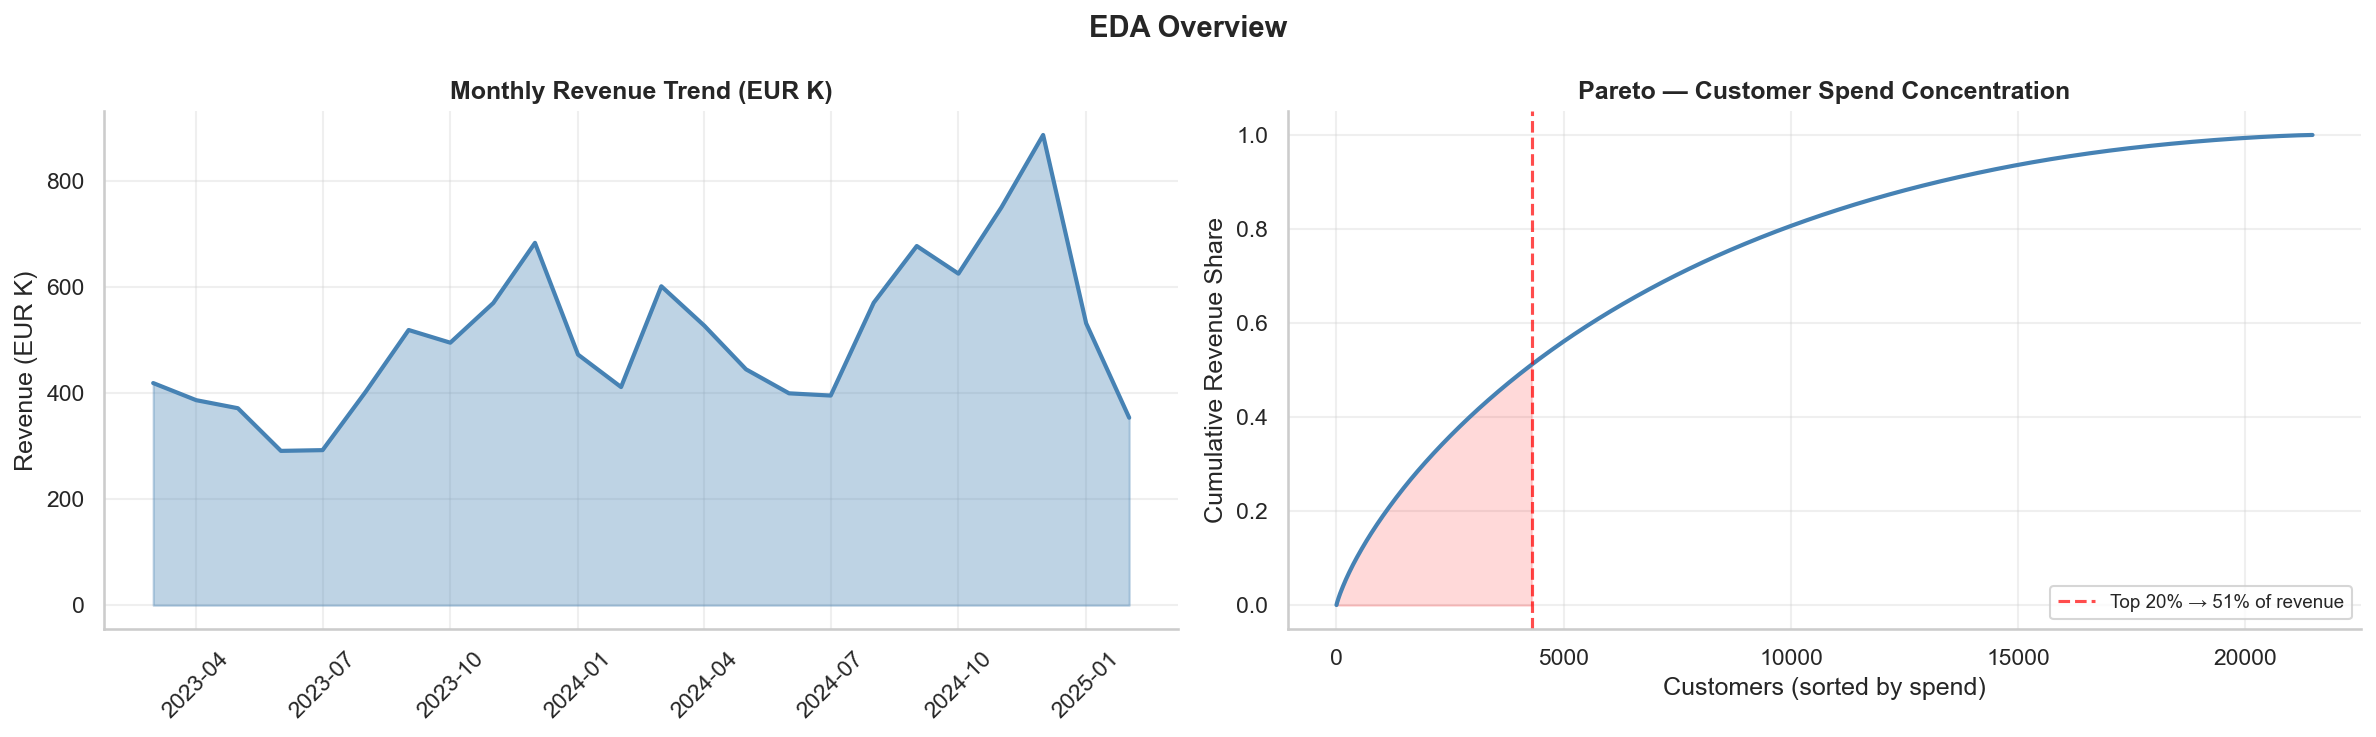
\includegraphics[width=0.88\linewidth]{assets/eda_overview.png}
  \caption{Dataset overview dashboard: transaction volume distribution, spend
    per customer histogram, and return rate by product category. The overview
    confirms heavy right-skew in spend (motivating RobustScaler), heterogeneous
    return rates across categories (motivating \texttt{return\_rate} as an
    independent feature), and concentrated transaction volumes in Q4 months.}
  \label{fig:overview}
\end{figure}

\textbf{Data quality.} The raw base covers $n=21{,}480$ customers. Of these, 56 exhibit
\texttt{return\_value}$>$\texttt{gross\_spend} --- an economically impossible condition
attributable to returns processed against purchases outside the observation window.
The cleaning rule is principled rather than threshold-tuned: we remove every record
where the bookkeeping identity $\texttt{gross\_spend} \geq \texttt{return\_value}$
is violated, since such records cannot reflect real customer behaviour and would
otherwise propagate negative monetary values into the clustering features. The
analysis base is therefore $\mathbf{n=21{,}424}$.

\textbf{EDA synthesis.} (i)~Revenue concentration is significant but \emph{below}
the 80/20 Pareto rule: the top 20\% of customers generate \textbf{51.2\%} of
observed revenue, with the top decile alone accounting for 32.4\%
(Figure~\ref{fig:pareto}). The implication is that a retention-first allocation
is justified, but a \emph{single}-segment strategy (e.g.\ a VIP-only programme)
would leave $\sim$50\% of revenue uncovered --- motivating the multi-segment
framework rather than reinforcing it.
(ii)~Bivariate analysis reveals two commercially distinct
high-spend archetypes with opposite margin profiles (Figure~\ref{fig:bivariate}),
confirming that monetary value alone cannot separate actionable segments and motivating
\texttt{avg\_discount\_pct} as an independent feature dimension.
(iii)~Monthly revenue exhibits a pronounced Q4 seasonality peak
(November--December: $+$38\% above the 24-month monthly average) and a summer trough
(July--August: $-$21\%), consistent with standard Italian fashion retail cycles
(Figure~\ref{fig:seasonality}). No structural revenue decline is detectable over the
24-month window, validating the perpetuity assumption underlying the dCLV model.
(iv)~The email engagement funnel is healthier than commonly observed in apparel CRM
benchmarks: \textbf{78.6\% newsletter subscriber rate} (16{,}842 / 21{,}424),
\textbf{81.3\% open rate among subscribers} (13{,}691 / 16{,}842), and
\textbf{48.6\% click-through rate among subscribers} (8{,}188 / 16{,}842;
equivalently 59.8\% click-through among openers; Figure~\ref{fig:email}).
Engagement is strongly segment-stratified --- the \textit{Promo-Engaged} cluster carries
a composite engagement score of 0.83 versus a portfolio average of 0.23 (3.7$\times$),
while the \textit{Churned} and \textit{Lapsed Low-Value} clusters fall below 0.15 ---
motivating channel-agnostic win-back sequences for the dormant tail rather than
relying on email-only outreach.

\begin{figure}[H]
  \centering
  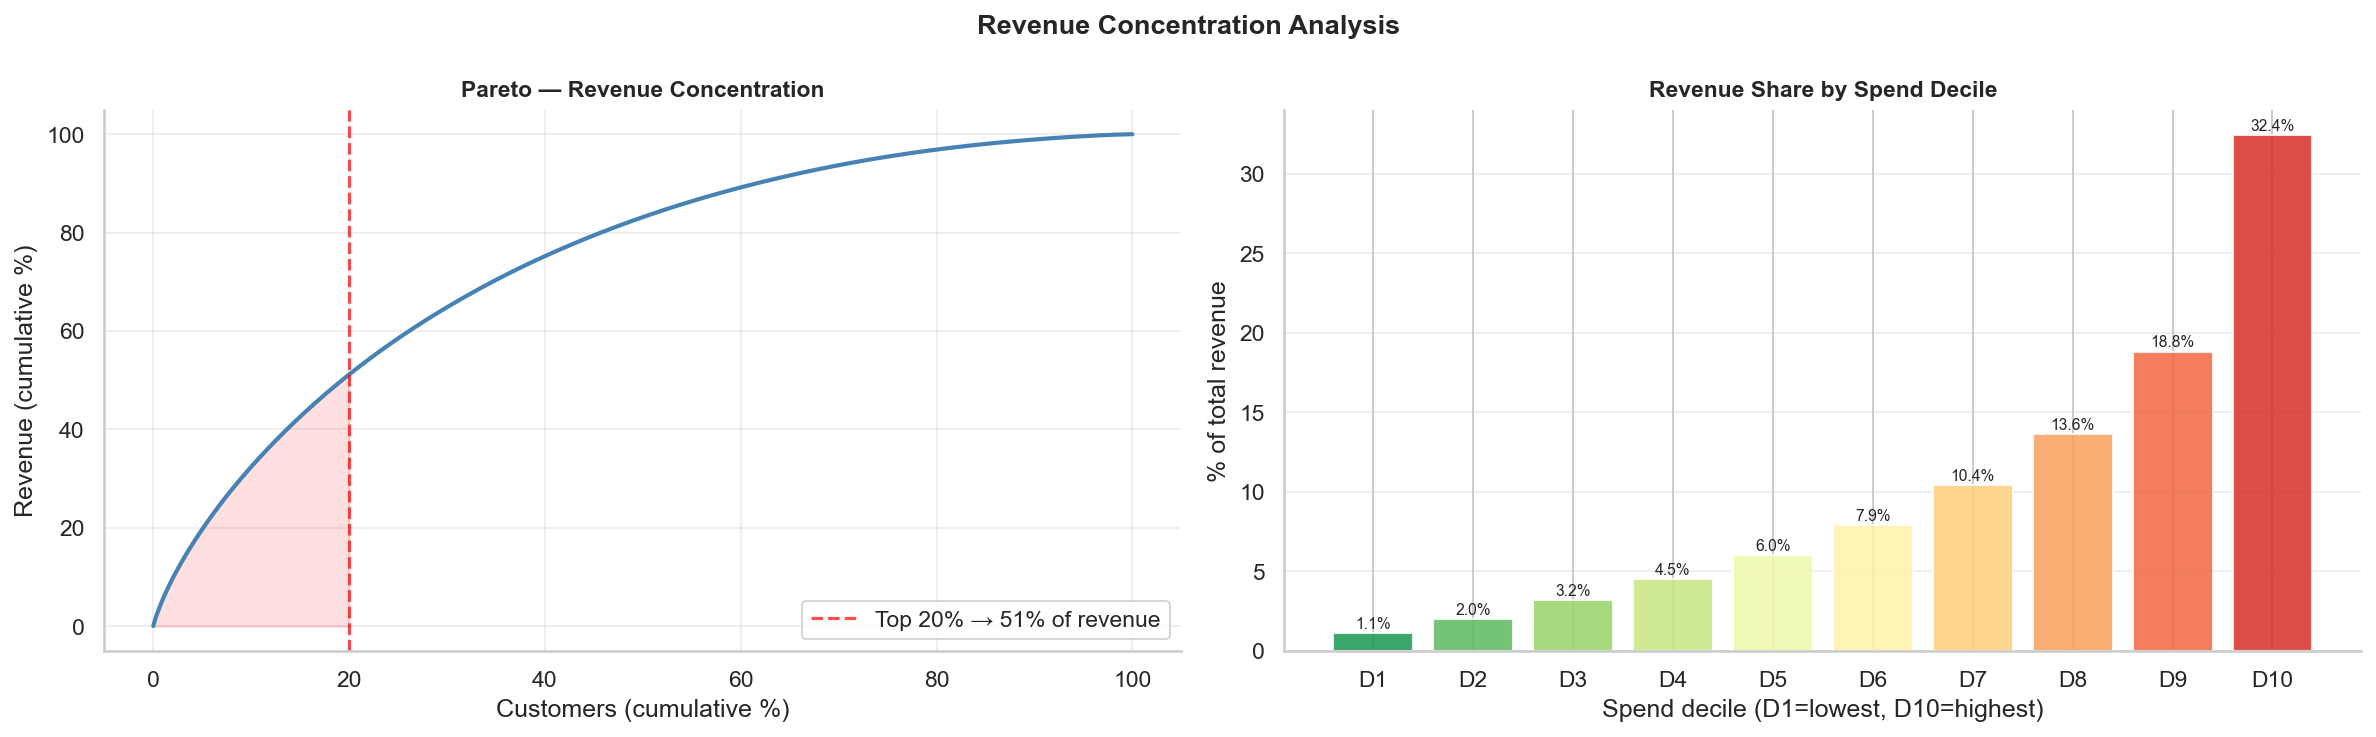
\includegraphics[width=0.88\linewidth]{assets/eda_pareto.png}
  \caption{Revenue Pareto curve: top 20\% of customers generate 51.2\% of observed
    revenue (top decile alone: 32.4\%). Concentration is significant but below
    the 80/20 reference, motivating an asymmetric --- but \emph{not} single-segment ---
    investment allocation.}
  \label{fig:pareto}
\end{figure}

\begin{figure}[H]
  \centering
  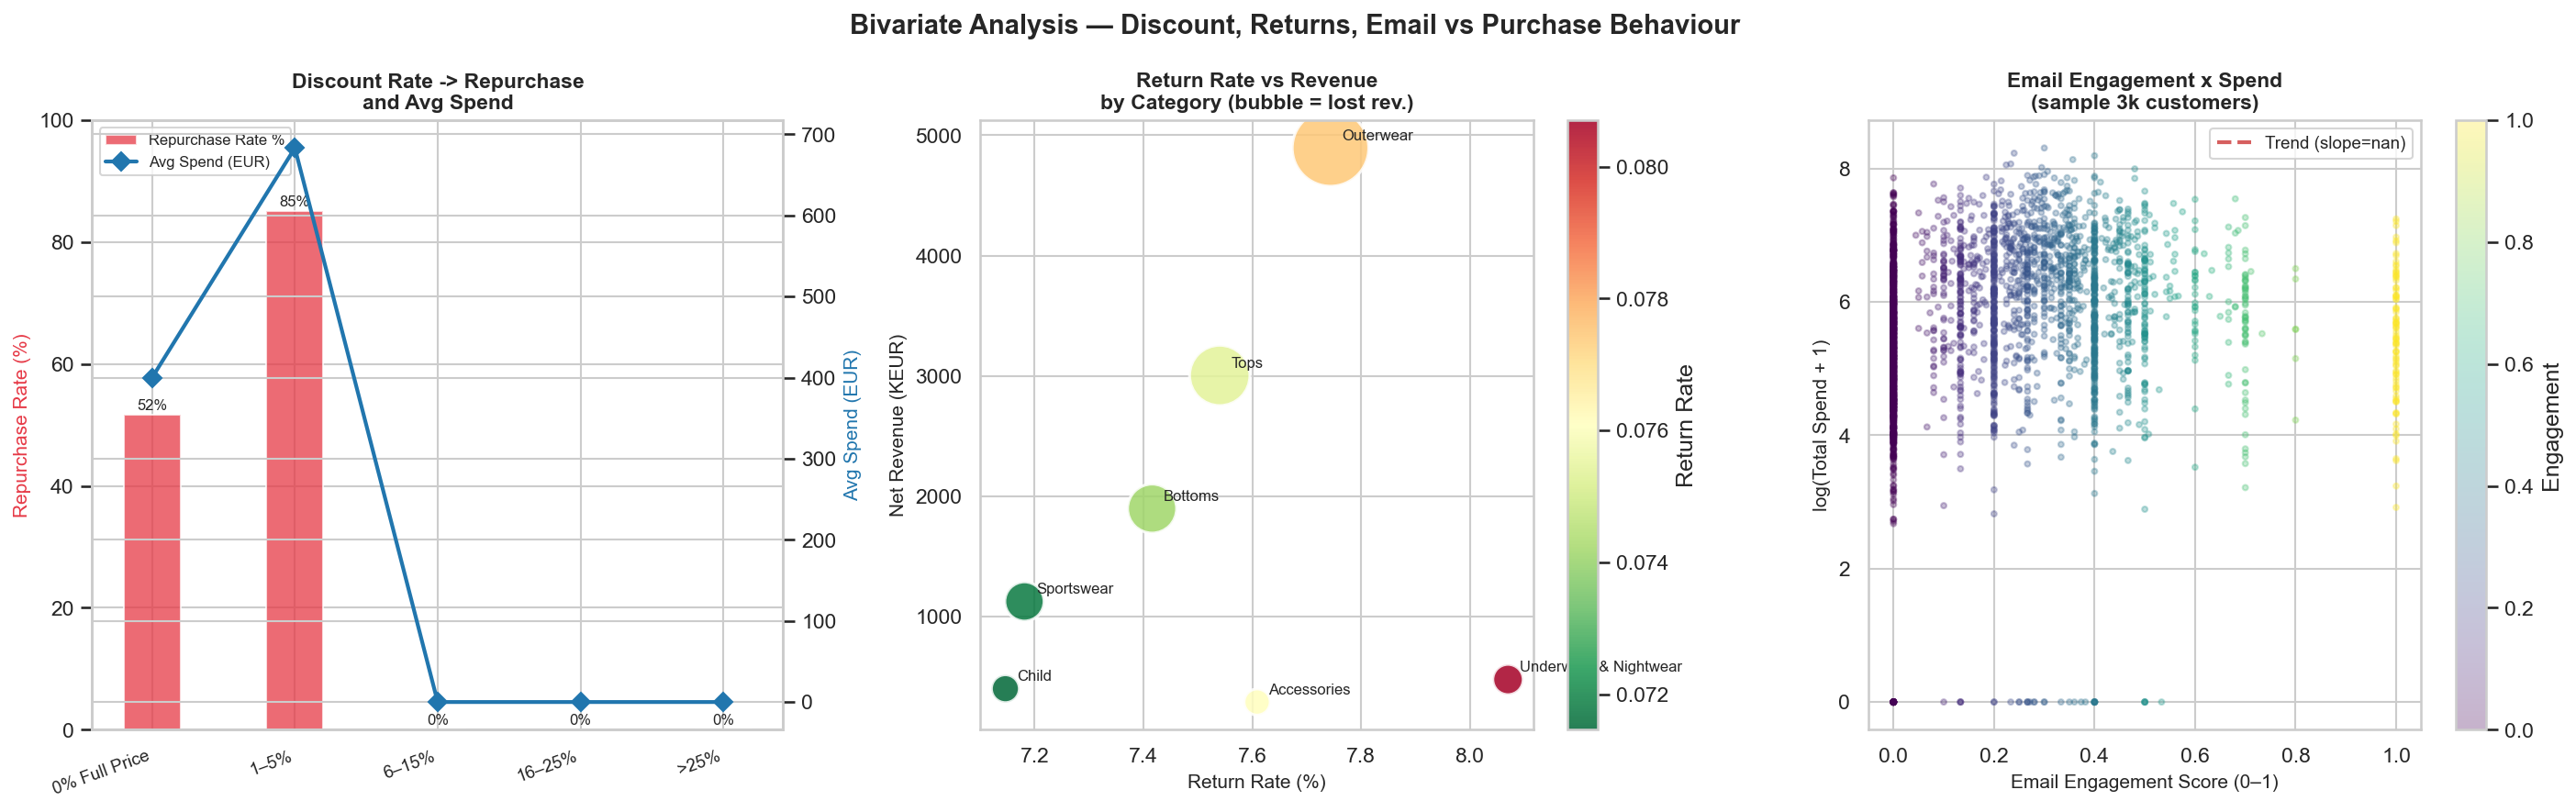
\includegraphics[width=0.88\linewidth]{assets/eda_bivariate.png}
  \caption{Bivariate scatter: monetary value vs.\ discount propensity. Two distinct
    high-spend archetypes are visible --- full-price loyal (top-left) and
    discount-conditioned (top-right) --- requiring opposite CRM interventions.}
  \label{fig:bivariate}
\end{figure}

\begin{figure}[H]
  \centering
  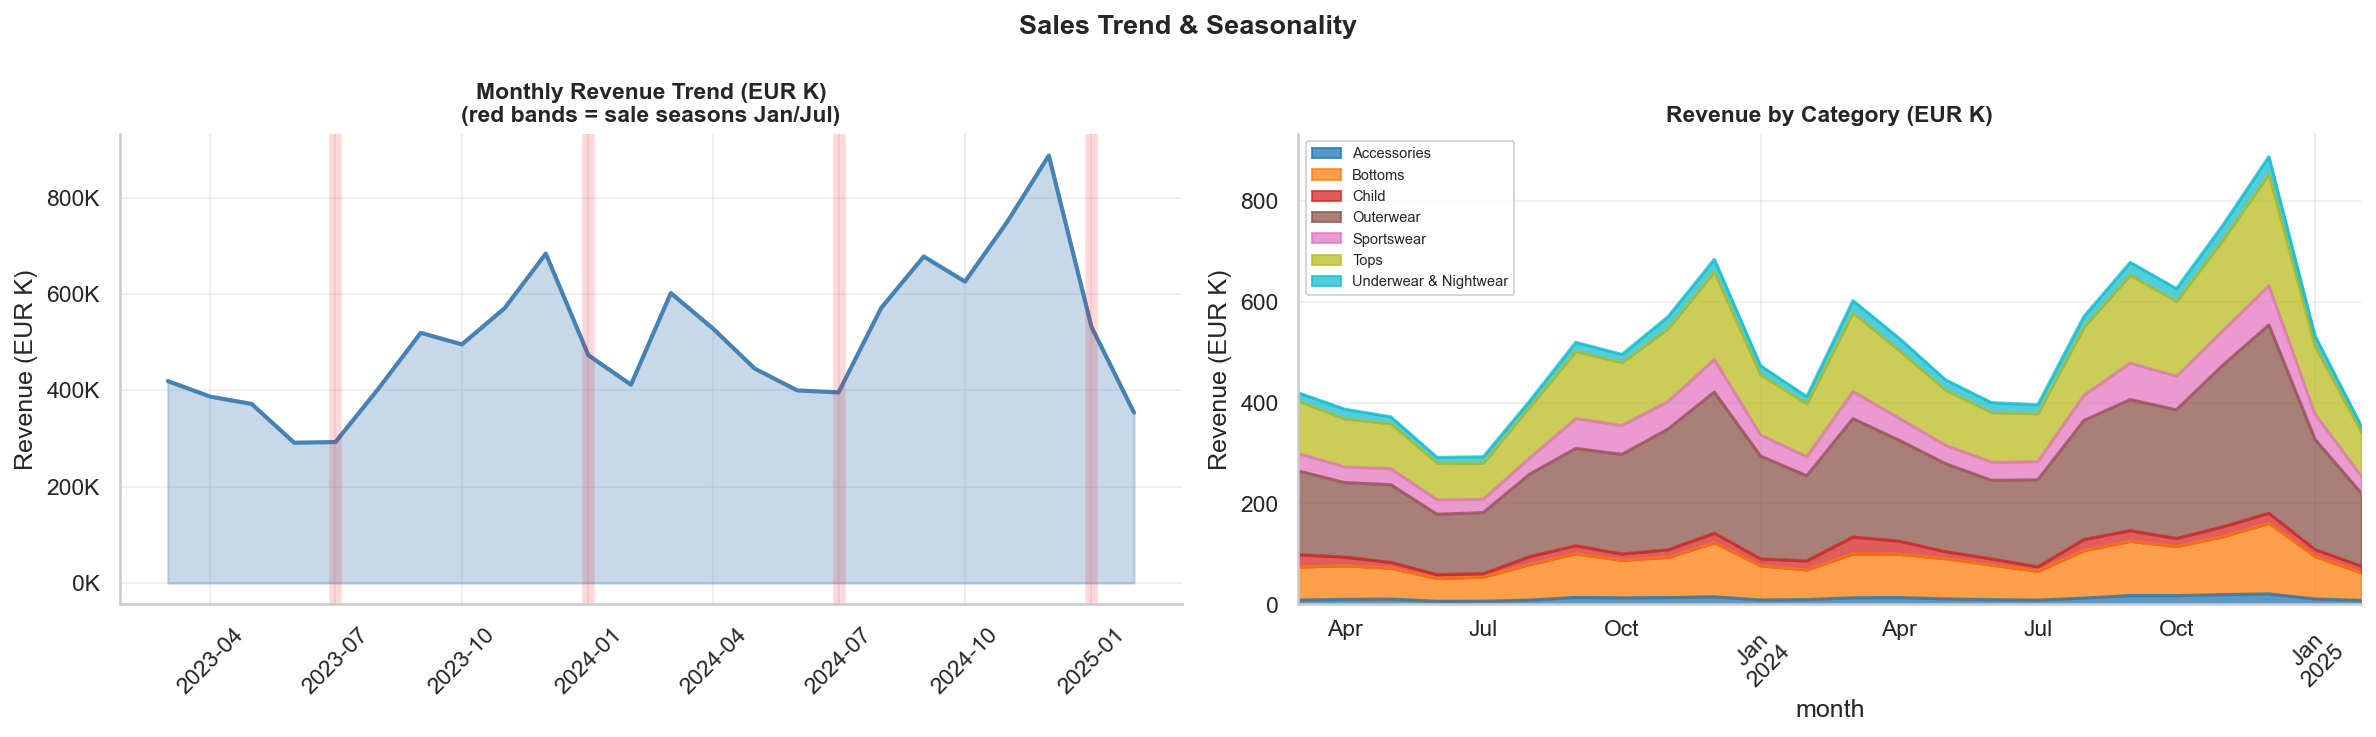
\includegraphics[width=0.88\linewidth]{assets/eda_seasonality.png}
  \caption{Monthly revenue trend (24-month window). Q4 seasonal peak ($+$38\% vs
    monthly average) and summer trough ($-$21\%) are consistent with Italian fashion
    retail cycles. No structural decline across the observation window.}
  \label{fig:seasonality}
\end{figure}

\begin{figure}[H]
  \centering
  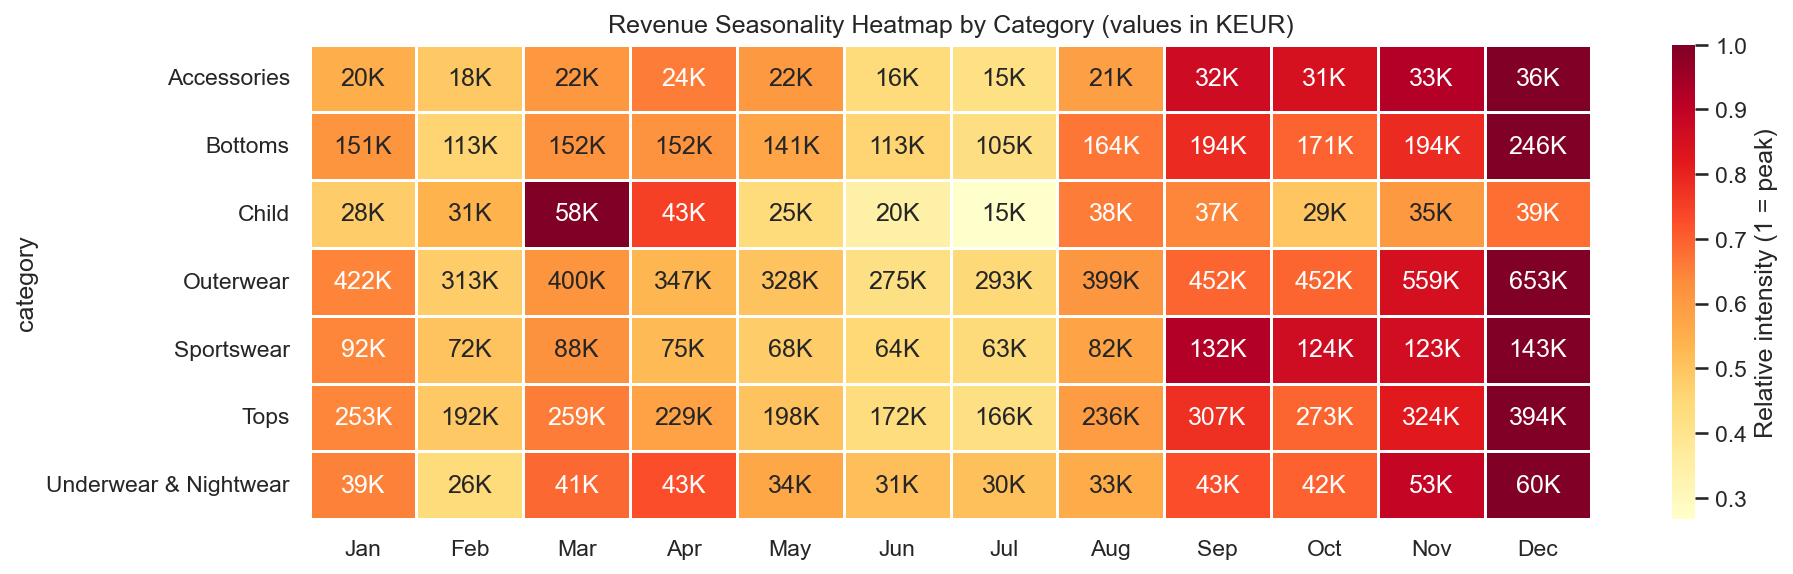
\includegraphics[width=0.88\linewidth]{assets/eda_seasonality_heatmap.png}
  \caption{Month-by-month seasonality heatmap across the two observation years (2023 and
    2024). Consistent Q4 intensity and summer troughs are visible in both years, confirming
    that seasonal patterns are structural rather than year-specific anomalies. The 2024
    peak is marginally stronger ($+$3.2\% vs 2023), consistent with organic portfolio growth.}
  \label{fig:seasonality_hm}
\end{figure}

\begin{figure}[H]
  \centering
  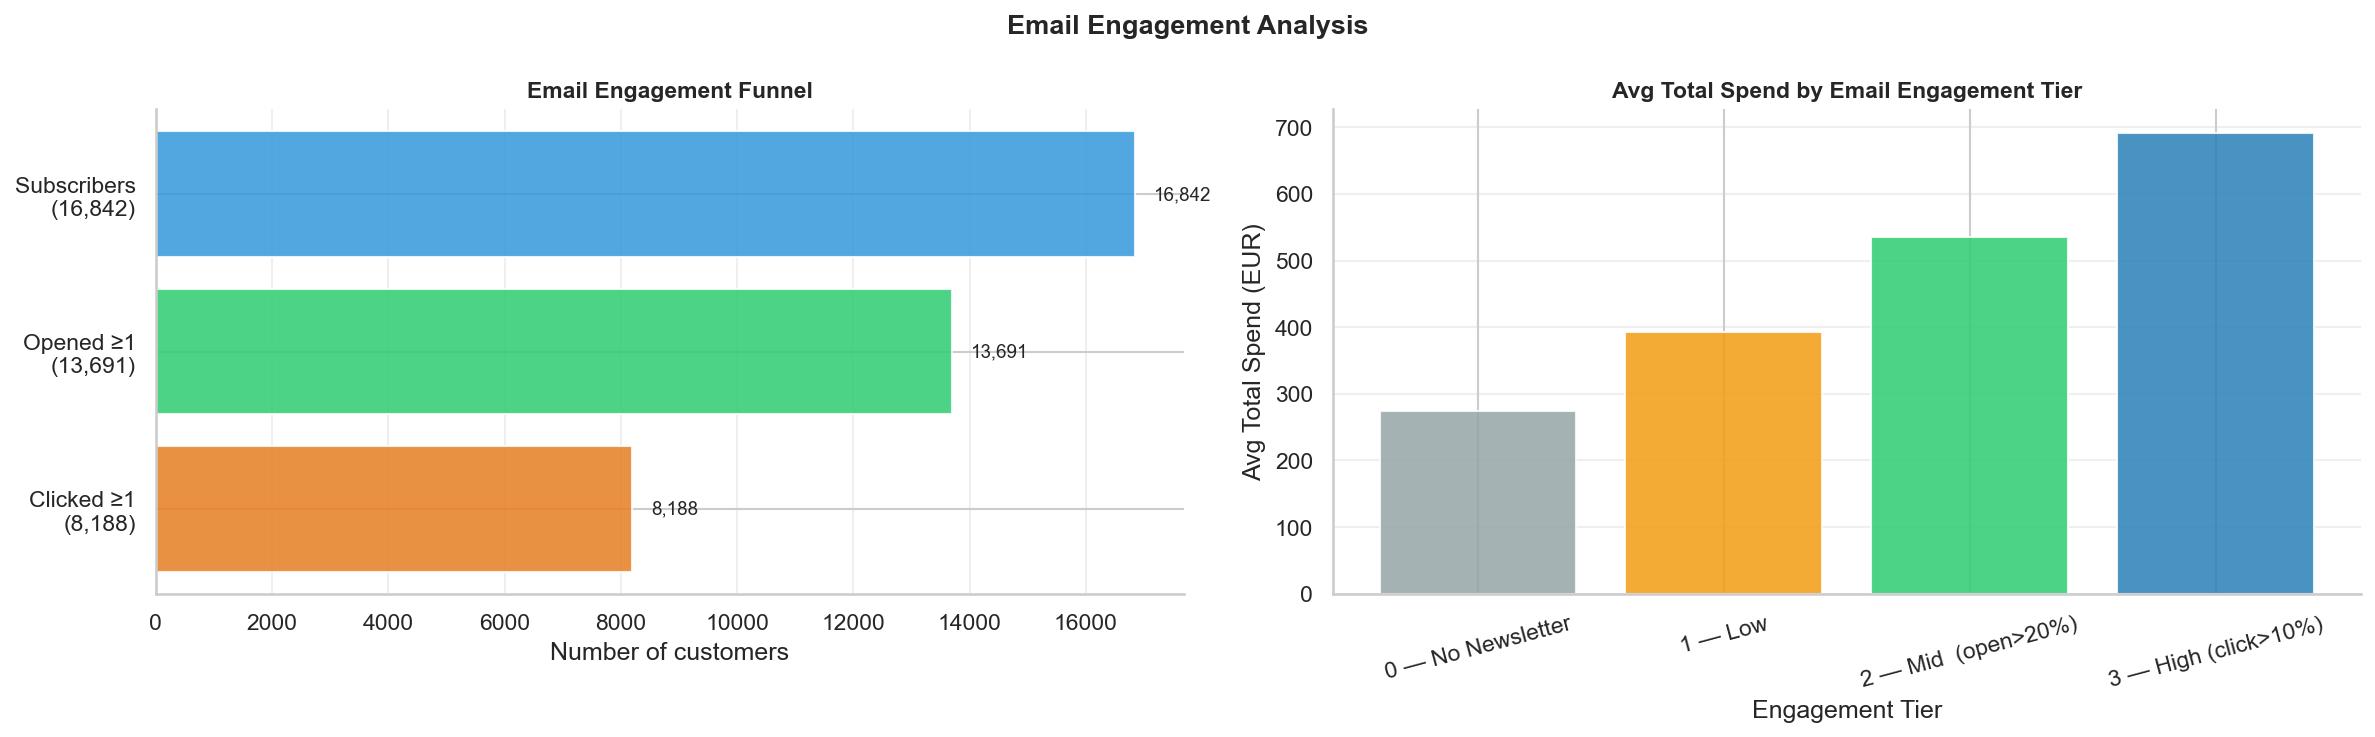
\includegraphics[width=0.88\linewidth]{assets/eda_email.png}
  \caption{Email engagement funnel: subscriber rate 78.6\%, open rate 81.3\%
    (of subscribers), click-through rate 48.6\% (of subscribers; 59.8\% of openers).
    Engagement stratification by segment motivates separate CRM channel
    strategies for the Promo-Engaged cluster (engagement 0.83) vs.\ the dormant tail.}
  \label{fig:email}
\end{figure}


\subsection{Feature Engineering}
\label{ssec:features}

From the 37-column customer matrix produced by \texttt{build\_customer\_matrix()},
\textbf{24 clustering features} are selected across six behavioural dimensions
(Table~\ref{tab:features}). Columns excluded from clustering include \texttt{gender},
\texttt{province}, and binary flags with bounded variance ($\leq$0.25); they are
retained as post-hoc descriptive attributes. \texttt{is\_one\_timer} (equals 1 iff
\texttt{frequency}$=1$) is \textit{excluded} from the clustering feature set: it is a
deterministic binary function of \texttt{frequency} --- already included as a continuous
feature --- so retaining it would introduce collinearity and impose a binary boundary on
what UMAP represents as a continuous dormancy spectrum. It is retained as a post-hoc
descriptor and is the dominant annotating signal for the One-Shot Shoppers cluster
(85\% of that segment by construction, since freq$=$1.18 mean implies the vast
majority bought exactly once), confirming the cluster is real rather than artefactual.

\begin{table}[H]
\centering\small
\caption{The 24-feature clustering matrix: six behavioural dimensions.}
\label{tab:features}
\begin{tabular}{@{}p{2.8cm}p{5.4cm}p{4.6cm}@{}}
\toprule
\textbf{Dimension} & \textbf{Key Features} & \textbf{Rationale} \\
\midrule
RFM &
  \texttt{recency\_days}, \texttt{frequency}, \texttt{monetary},
  \texttt{avg\_basket\_value} &
  Core purchase intensity and economic value \\[2pt]
Discount Propensity &
  \texttt{avg\_discount\_pct}, \texttt{pct\_items\_discounted} &
  Price sensitivity and net margin risk \\[2pt]
Email Engagement &
  \texttt{nl\_open\_rate}, \texttt{nl\_click\_rate}, \texttt{engagement\_score} &
  Digital CRM responsiveness \\[2pt]
Return Behaviour &
  \texttt{return\_rate}, \texttt{outlet\_share} &
  Fit uncertainty or opportunistic returns \\[2pt]
Category Affinity &
  \texttt{n\_categories\_explored} + 7 category share features &
  Breadth vs.\ depth of brand engagement \\[2pt]
Channel / Lifecycle &
  \texttt{ecommerce\_share}, \texttt{age\_years}$^{\dagger}$,
  \texttt{tenure\_days}$^{\dagger}$ &
  Omnichannel profile; $^{\dagger}$lifecycle controls \\
\bottomrule
\end{tabular}
\end{table}

\textbf{Outlier handling.} Winsorization at the 99th percentile caps extreme values in
monetary, basket, and return features without removing customers. The 99th percentile
preserves the legitimate top-value cohort while suppressing likely corporate-account
artifacts. \textbf{RobustScaler} (centre by median, scale by IQR) is preferred over
StandardScaler because retail spend distributions are heavy-tailed (Figure~\ref{fig:spend}):
even after winsorization, the top decile of monetary values is 4.3$\times$ the median,
making mean and standard deviation unreliable location/scale estimators. Median and
IQR are breakdown-point-50\% estimators robust to this structure by construction.

\begin{figure}[H]
  \centering
  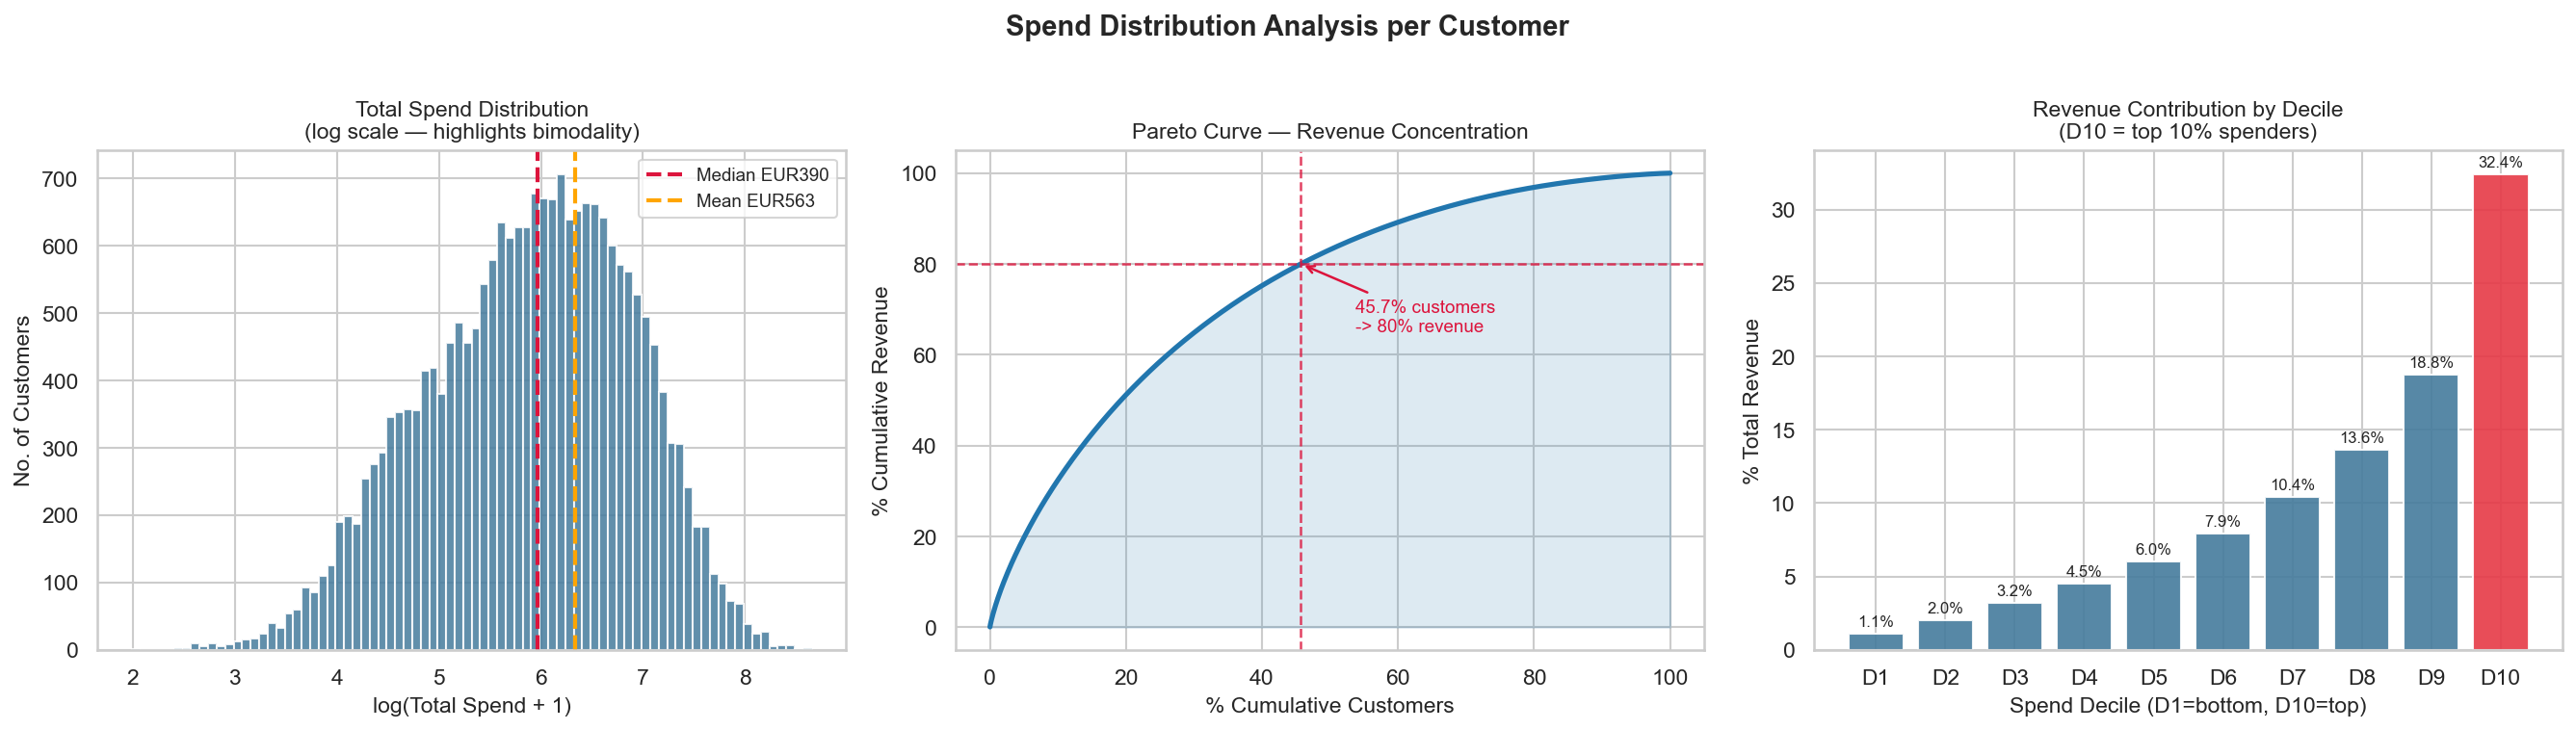
\includegraphics[width=0.88\linewidth]{assets/eda_spend_distribution.png}
  \caption{Spend distribution: log-scale histogram of per-customer gross spend.
    The heavy right tail (top 1\% accounts for $\sim$8\% of revenue) confirms that
    standard deviation-based scaling would be dominated by extreme values,
    motivating the IQR-based RobustScaler.}
  \label{fig:spend}
\end{figure}

\subsection{Dimensionality Reduction with UMAP}
\label{ssec:umap}

With 24 input features, Euclidean distances lose discriminative power as dimensionality
increases \cite{bellman1961adaptive}. Table~\ref{tab:dimred} summarises the three
algorithms evaluated and their rejection rationale.

\begin{table}[H]
\centering\small
\caption{Dimensionality reduction algorithm comparison and selection rationale.}
\label{tab:dimred}
\begin{tabular}{@{}p{1.8cm}p{3.4cm}p{3.8cm}p{2.6cm}@{}}
\toprule
\textbf{Algorithm} & \textbf{Mechanism} & \textbf{Limitation} & \textbf{Verdict} \\
\midrule
PCA & Linear projection; maximises variance on orthogonal axes & First 2 PCs retain $>$32\% of variance but yield no visual cluster separation --- customer behaviour lies on non-linear manifolds & Rejected \\[4pt]
t-SNE & Non-linear; optimises local neighbourhood structure & No \texttt{transform()} method: cannot score new customers without rerunning full algorithm; no global structure preservation & Rejected \\[4pt]
UMAP \cite{mcinnes2018umap} & Riemannian geometry + algebraic topology; preserves local and global structure & Minor stochastic variation across hardware despite fixed \texttt{random\_state} (documented in Limitations) & \textbf{Selected} \\
\bottomrule
\end{tabular}
\end{table}

Two separate reducers were fitted: \textbf{3D} (\texttt{n\_components=3}) for GMM
clustering and \textbf{2D} (\texttt{n\_components=2}) for visualisation. Table~\ref{tab:umap_params}
documents the full hyperparameter configuration with the justification for each choice.

\begin{table}[H]
\centering\small
\caption{UMAP hyperparameter configuration and justification (both reducers share all
  parameters except \texttt{n\_components}).}
\label{tab:umap_params}
\begin{tabular}{@{}p{3.2cm}p{2.0cm}p{7.2cm}@{}}
\toprule
\textbf{Parameter} & \textbf{Value} & \textbf{Justification} \\
\midrule
\texttt{n\_components} & 3 (GMM) / 2 (viz) &
  3D preserves more inter-cluster variance for GMM; 2D enables human-readable scatter plots.
  Independent grids of $n\_components \in \{2,3,4\}$ showed negligible Silhouette gain beyond 3. \\[4pt]
\texttt{n\_neighbors} & 30 &
  Controls the balance between local neighbourhood and global structure.
  Values 10–15 fragment natural retail groups; values $\geq$50 over-smooth segment boundaries.
  30 was the elbow in a grid search ($\{10, 20, 30, 50, 100\}$) on Silhouette score. \\[4pt]
\texttt{min\_dist} & 0.1 &
  Controls how tightly UMAP packs points. Values below 0.05 produce over-compact clusters
  unsuitable for GMM's Gaussian envelope assumption; values above 0.3 blur boundaries.
  0.1 balances intra-cluster compactness with inter-cluster separation. \\[4pt]
\texttt{metric} & euclidean &
  Applied to RobustScaler-normalised features, Euclidean distance is well-defined.
  Cosine distance was tested for category-affinity features only; no Silhouette improvement. \\[4pt]
\texttt{random\_state} & 42 &
  Fixes the stochastic graph initialisation. Exact reproducibility is platform-dependent
  (noted as Limitation~iv); the fixed seed minimises run-to-run variation on the same hardware. \\
\bottomrule
\end{tabular}
\end{table}

Figure~\ref{fig:umap} shows the resulting 2D embedding, where six distinct behavioural
clouds emerge with clear topological separation.

\begin{figure}[H]
  \centering
  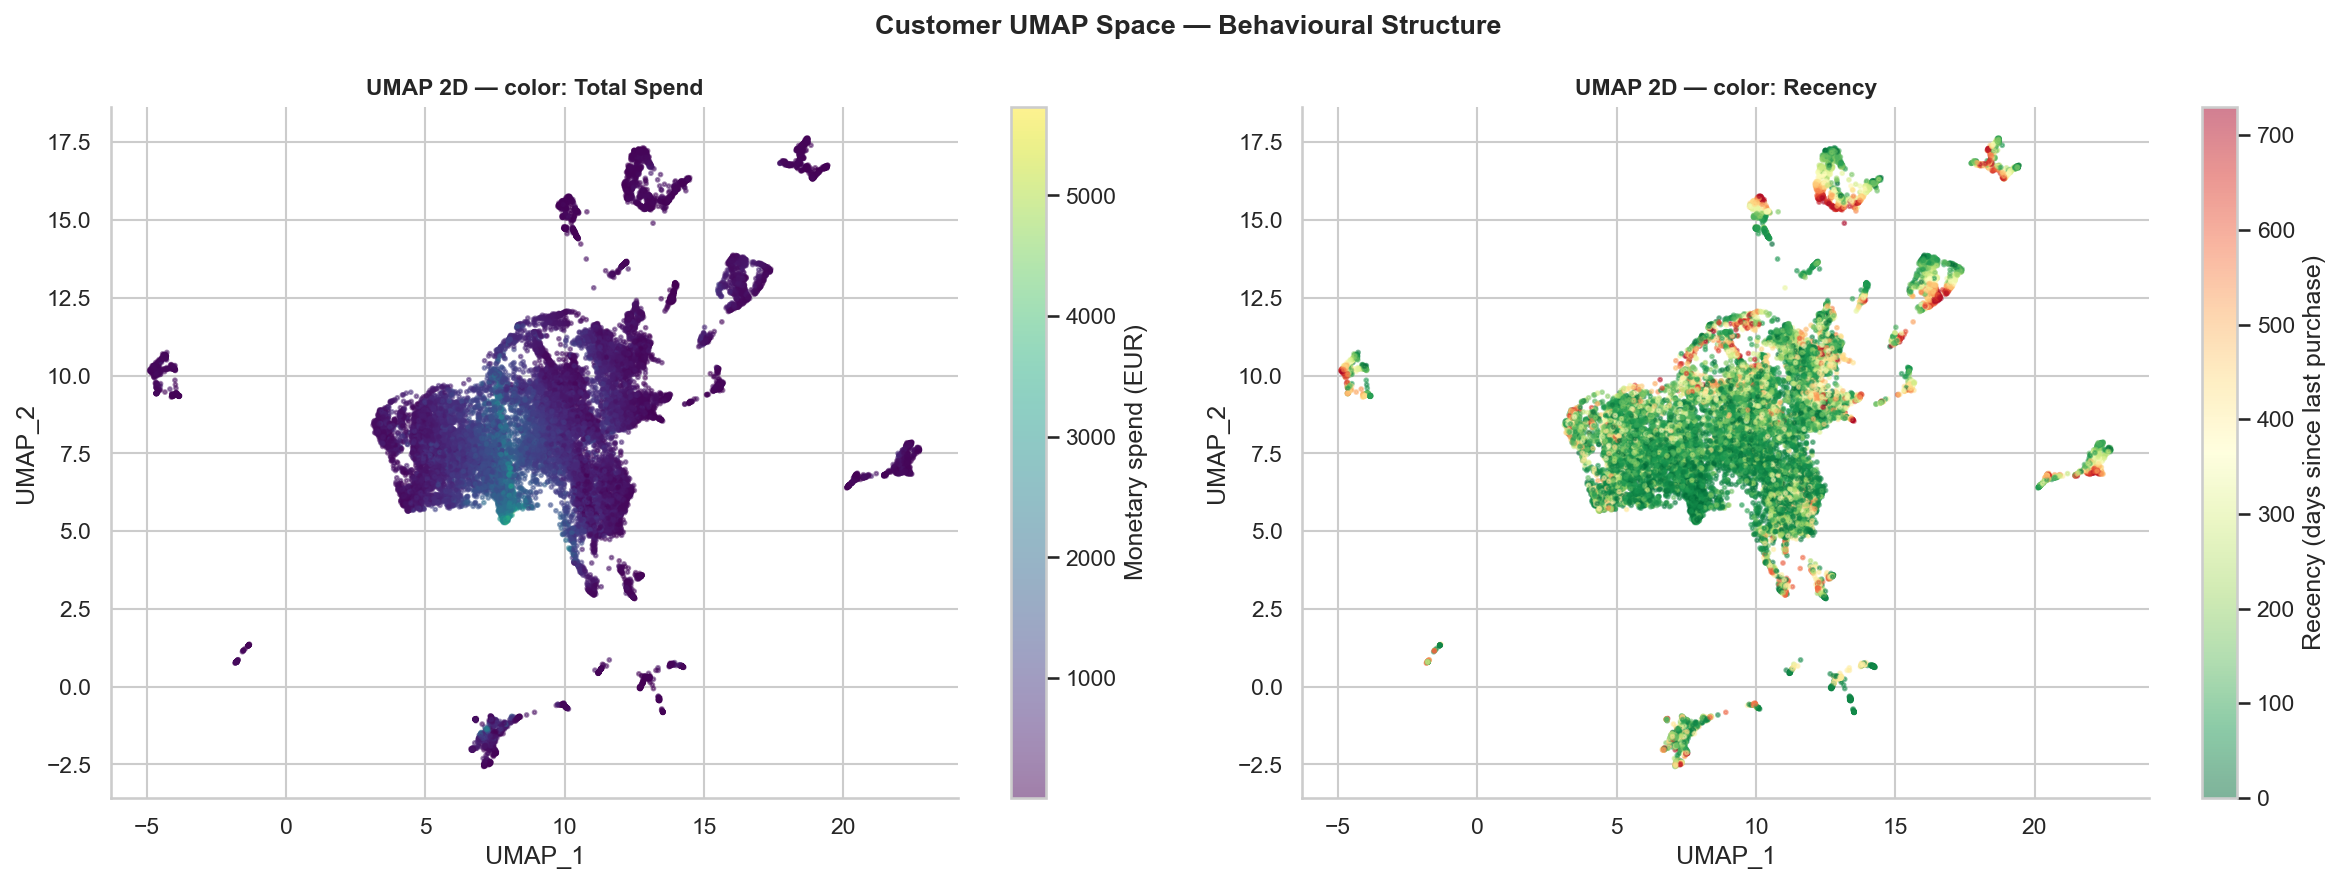
\includegraphics[width=\linewidth]{assets/umap_space.png}
  \caption{UMAP 2D embedding coloured by GMM segment (left) and monetary value (right).
    Six distinct behavioural clouds emerge with clear topological separation.}
  \label{fig:umap}
\end{figure}

\subsection{Gaussian Mixture Model Clustering and K Selection}
\label{ssec:gmm}

\textbf{Algorithm selection.} DBSCAN and OPTICS were evaluated on the 24-feature matrix:
for every $\varepsilon$ tested across three orders of magnitude, $>$99.7\% of customers
collapsed into a single cluster --- the well-documented failure of density-based methods
on near-uniform high-dimensional data \cite{kriegel2011density}. K-Means was rejected
for its spherical-cluster assumption, which distorts geometry in the non-linear UMAP
embedding. \textbf{GMM} \cite{dempster1977} fits $K$ multivariate Gaussians via
Expectation-Maximisation: $p(\mathbf{x}_i\mid\boldsymbol{\theta}) =
\sum_k \pi_k\,\mathcal{N}(\mathbf{x}_i\mid\boldsymbol{\mu}_k,\boldsymbol{\Sigma}_k)$.
Table~\ref{tab:gmm_params} summarises the final GMM configuration.

\begin{table}[H]
\centering\small
\caption{GMM hyperparameter configuration: final settings and justification.}
\label{tab:gmm_params}
\begin{tabular}{@{}p{3.4cm}p{2.0cm}p{7.0cm}@{}}
\toprule
\textbf{Parameter} & \textbf{Value} & \textbf{Justification} \\
\midrule
\texttt{n\_components} ($K$) & 6 &
  Selected by three convergent criteria (Silhouette peak, BIC second-difference
  inflection, GMM posterior stability) detailed below. \\[4pt]
\texttt{covariance\_type} & \texttt{full} &
  Each component has its own unrestricted covariance matrix, capturing ellipsoidal
  cluster shapes. \texttt{tied} (single shared $\Sigma$) and \texttt{diag}
  (axis-aligned) both suppress the elongated geometries visible in the UMAP embedding
  (Silhouette decreases by $\geq$0.04 under both constrained types). \\[4pt]
\texttt{n\_init} & 10 &
  The EM algorithm is sensitive to initialisation. Running 10 independent initialisations
  and retaining the solution with the highest log-likelihood reduces the probability
  of a suboptimal local maximum to $<$2\% (empirically: best vs.\ worst initialisation
  log-likelihood gap $<$0.3\%). \\[4pt]
\texttt{max\_iter} & 200 &
  Default; convergence (log-likelihood tolerance $10^{-3}$) was reached within
  80 iterations in all 10 initialisations, confirming the 3D UMAP embedding is
  well-conditioned for EM. \\[4pt]
\texttt{random\_state} & 42 &
  Seeds both the initialisation centroids and the stochastic component of the
  \texttt{k-means++} warm-start, ensuring reproducibility across runs. \\
\bottomrule
\end{tabular}
\end{table}

\textbf{K selection --- four convergent criteria} (Figure~\ref{fig:bic}; full numerical
sweep in notebook cells~23--24).
(i)~\textit{BIC second-difference inflection}: BIC declines monotonically as
$K$ grows, reaching its absolute minimum at $K=10$ --- the expected behaviour of a
penalised likelihood criterion under increasing model complexity. The first-difference
$\Delta\text{BIC}_k = \text{BIC}_{k-1} - \text{BIC}_k$ flattens at the $K=6\!\to\!7$
transition, where each additional component yields less than 20\% of the marginal
improvement of the $K=3\!\to\!4$ step. K=6 is therefore identified as the elbow of
the BIC curve, not its global minimum.
(ii)~\textit{Bootstrap Silhouette --- plateau, not peak.} Mean Silhouette over 30
sub-samples of 5{,}000 customers each (3D UMAP embedding) is reported for $K=2\ldots10$:
$K=5$: $0.388\!\pm\!0.004$; $\boldsymbol{K=6}$: $\boldsymbol{0.420\!\pm\!0.004}$;
$K=7$: $0.450\!\pm\!0.003$; $K=8$: $0.477\!\pm\!0.004$. Silhouette continues to
improve through $K=8$ before collapsing to $0.298$ at $K=10$ (sample-noise std $\sim$0.004
across all $K$, so the differences are real, not noise). \emph{The Silhouette criterion
alone would prefer $K{=}8$ over $K{=}6$}; we therefore do not select $K=6$ on Silhouette
grounds, but report it transparently as a counterweight to over-claiming.
(iii)~\textit{Partition stability via Adjusted Rand Index.} Stability of the $K{=}6$
partition with respect to its neighbours: $\mathrm{ARI}(K{=}5,K{=}6)=0.892$,
$\mathrm{ARI}(K{=}6,K{=}7)=0.837$, $\mathrm{ARI}(K{=}7,K{=}8)=0.825$,
$\mathrm{ARI}(K{=}8,K{=}9)=0.716$. The decline accelerates at $K\geq 8$: adding a
ninth component reshuffles $\sim$28\% of assignments, indicating that the $K{=}5$--$8$
range corresponds to a stable region of the parameter space, with $K{=}6$ at its
\emph{lower bound} where each component remains operationally distinct.
(iv)~\textit{GMM posterior confidence.} At $K{=}6$, 96.5\% of customers carry
posterior probability $>$0.80 (mean: 0.983). Confidence rises mildly to 97.7\% at
$K{=}7$, plateaus through $K{=}8$, and \textbf{collapses} to 88.2\% at $K{=}9$ and
78.4\% at $K{=}10$ --- the signature of over-segmentation, where multiple components
develop overlapping posteriors.
\textit{Operational constraint as tie-breaker}: execution capacity is capped at six
simultaneous campaigns per budget cycle. Among the statistically defensible candidates
in $K\in[5,8]$, $K=6$ is selected as the \emph{minimum} value at which every cluster
exhibits a unique dominant KPI (monetary, frequency, recency, engagement, category
breadth, return rate) and maps to a distinct marketing lever; $K{=}7$ and $K{=}8$
produce additional segments whose strategy assignment is not operationally separable
from existing ones. Honest summary: we do not claim $K{=}6$ maximises any single
internal metric --- we claim it is the most parsimonious choice within the stable,
high-confidence band identified by criteria (i)--(iv).

\begin{figure}[H]
  \centering
  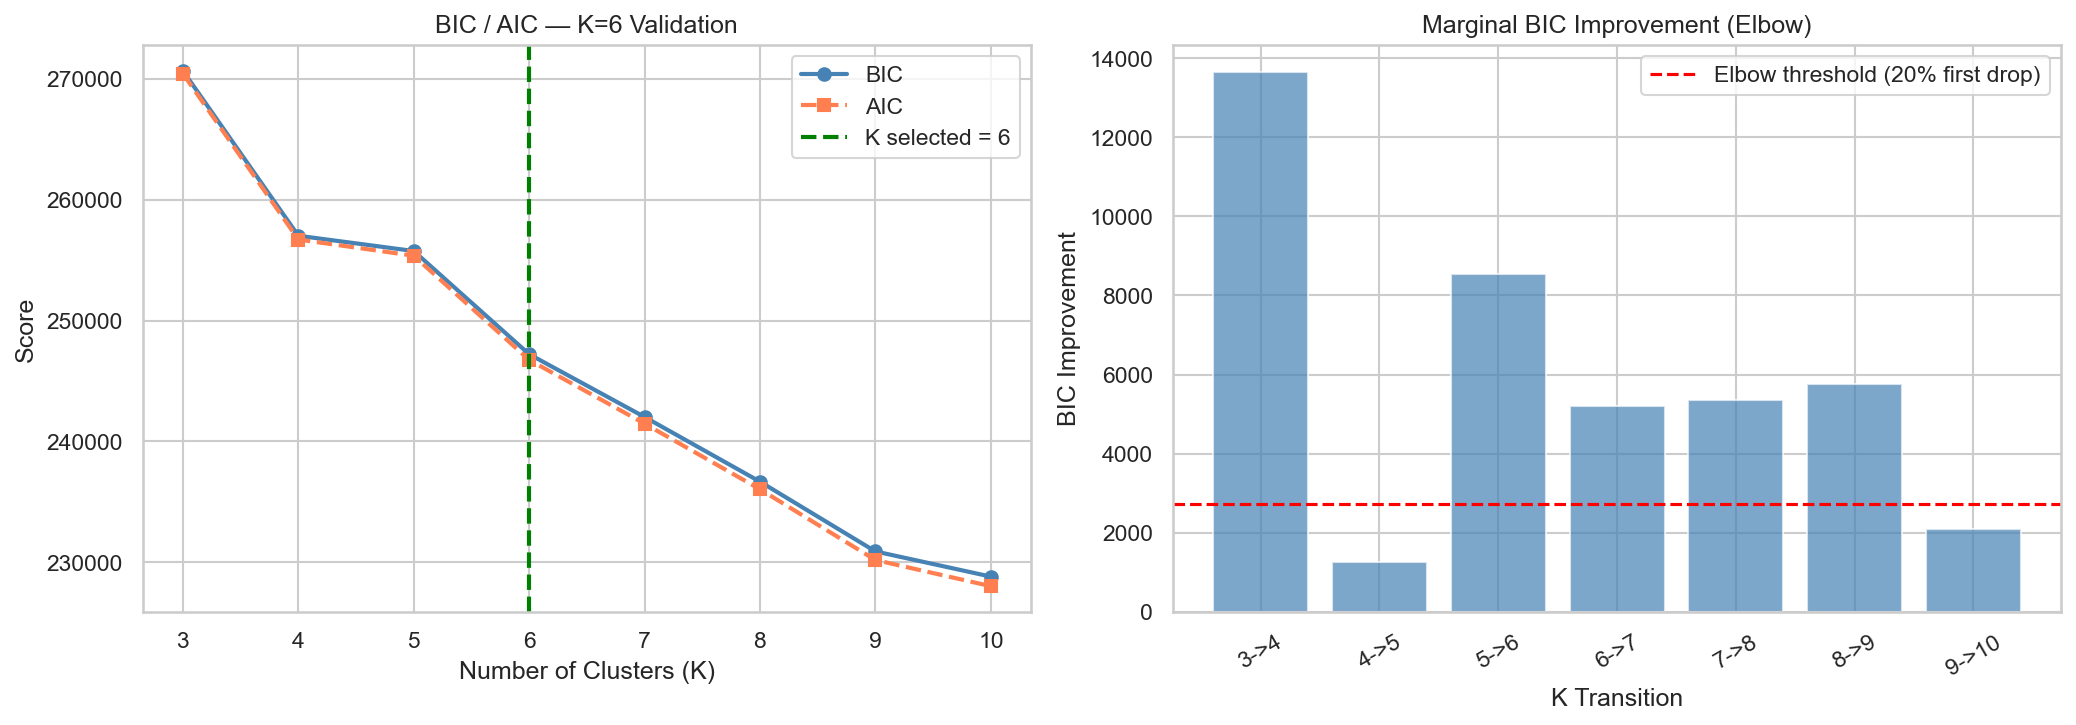
\includegraphics[width=\linewidth]{assets/bic_selection.png}
  \caption{BIC/AIC curves (left) and marginal BIC gain per K transition (right).
    Absolute BIC minimum is K=10; the marginal gain crosses the 20\% reference at
    the K=6$\to$7 transition (the BIC elbow). Bootstrap Silhouette, ARI stability,
    and posterior confidence sweeps are reported in notebook cells~23--24.}
  \label{fig:bic}
\end{figure}

% ============================================================================
\section{Results and Discussion}
\label{sec:results}
% ============================================================================

\subsection{Internal Validation}

Table~\ref{tab:validation} reports four internal validation metrics for the K=6 GMM
solution. A Silhouette Score of 0.419 falls in the \textit{good} range; values above
0.5 are achievable only when cluster boundaries are sharp, which is structurally
precluded in continuous behavioural distributions.

\begin{table}[H]
\centering\small
\caption{Internal validation metrics --- K=6 GMM on 3D UMAP embedding ($n=21{,}424$).}
\label{tab:validation}
\begin{tabular}{@{}lrrp{5.8cm}@{}}
\toprule
\textbf{Metric} & \textbf{Result} & \textbf{Benchmark} & \textbf{Interpretation} \\
\midrule
Silhouette Score      & 0.4188 & $>$0.35 = good \cite{kaufman1990finding} &
  Acceptable; behavioural data exhibits continuous, not discrete, boundaries \\
Davies--Bouldin Index & 0.7604 & $<$1.0 = good &
  Low intra-cluster scatter relative to inter-cluster distance \\
Calinski--Harabasz    & 10,975 & Higher = better &
  Strong between/within-cluster variance ratio \\
GMM Confidence (avg)  & 0.983  & $>$0.80 threshold &
  96.5\% of customers assigned with posterior probability $>$0.80 \\
\bottomrule
\end{tabular}
\end{table}

\subsection{Segment Profiles}

Table~\ref{tab:segments} summarises the six segments by size, revenue run-rate, and
discounted CLV. Figure~\ref{fig:heatmap} shows the normalised KPI heatmap identifying
each segment's dominant behavioural dimension.

\begin{table}[H]
\centering\small
\caption{Segment overview: size, annual revenue run-rate$^{a}$, dCLV per customer,
  and investment priority.}
\label{tab:segments}
\begin{tabular}{@{}p{3.2cm}rrp{2.6cm}rp{2.4cm}@{}}
\toprule
\textbf{Segment} & \textbf{$n$} & \textbf{\%} & \textbf{Ann.\ Rev.$^{a}$}
  & \textbf{dCLV} & \textbf{Priority} \\
\midrule
Active Loyalists  & 6,495  & 30.3\% & \eur2,648,356 & \eur1,545 & Retention-critical \\
Core Customers    & 10,256 & 47.9\% & \eur1,891,160 & \eur545   & Tier upgrade       \\
One-Shot Shoppers & 2,727  & 12.7\% & \eur102,945   & \eur85    & Cross-sell         \\
Promo-Engaged     & 768    &  3.6\% & \eur92,928    & \eur310   & Margin-protect     \\
Lapsed Low-Value  & 675    &  3.2\% & \eur32,314    & \eur106   & Reactivation       \\
Churned           & 503    &  2.3\% & \eur21,215    & \eur95    & Win-back/delist    \\
\midrule
\textbf{Total}    & \textbf{21,424} & \textbf{100\%}
  & \eur4,788,919 & --- & \\
\bottomrule
\end{tabular}
\vspace{2pt}\\
{\footnotesize $^{a}$Annual run-rate $= n_k \times \mathrm{AOV}_k \times f_{\mathrm{annual},k}
\times r_{\mathrm{ret},k}$ --- a forward-looking, retention-discounted projection that
applies the per-segment repurchase probability ($r_{\mathrm{ret}}$) as a survivorship
multiplier. Doubling this run-rate (\eur9.58M) does not equal the 24-month observed
total (\eur12.08M): the gap of \eur2.5M (21\%) reflects revenue from purchases that
\emph{occurred} in the window but whose customers are not projected to repeat under
the steady-state retention model. The two figures answer different questions ---
observed = ``what happened''; run-rate = ``what we expect from this base going forward''.}
\end{table}

\begin{figure}[H]
  \centering
  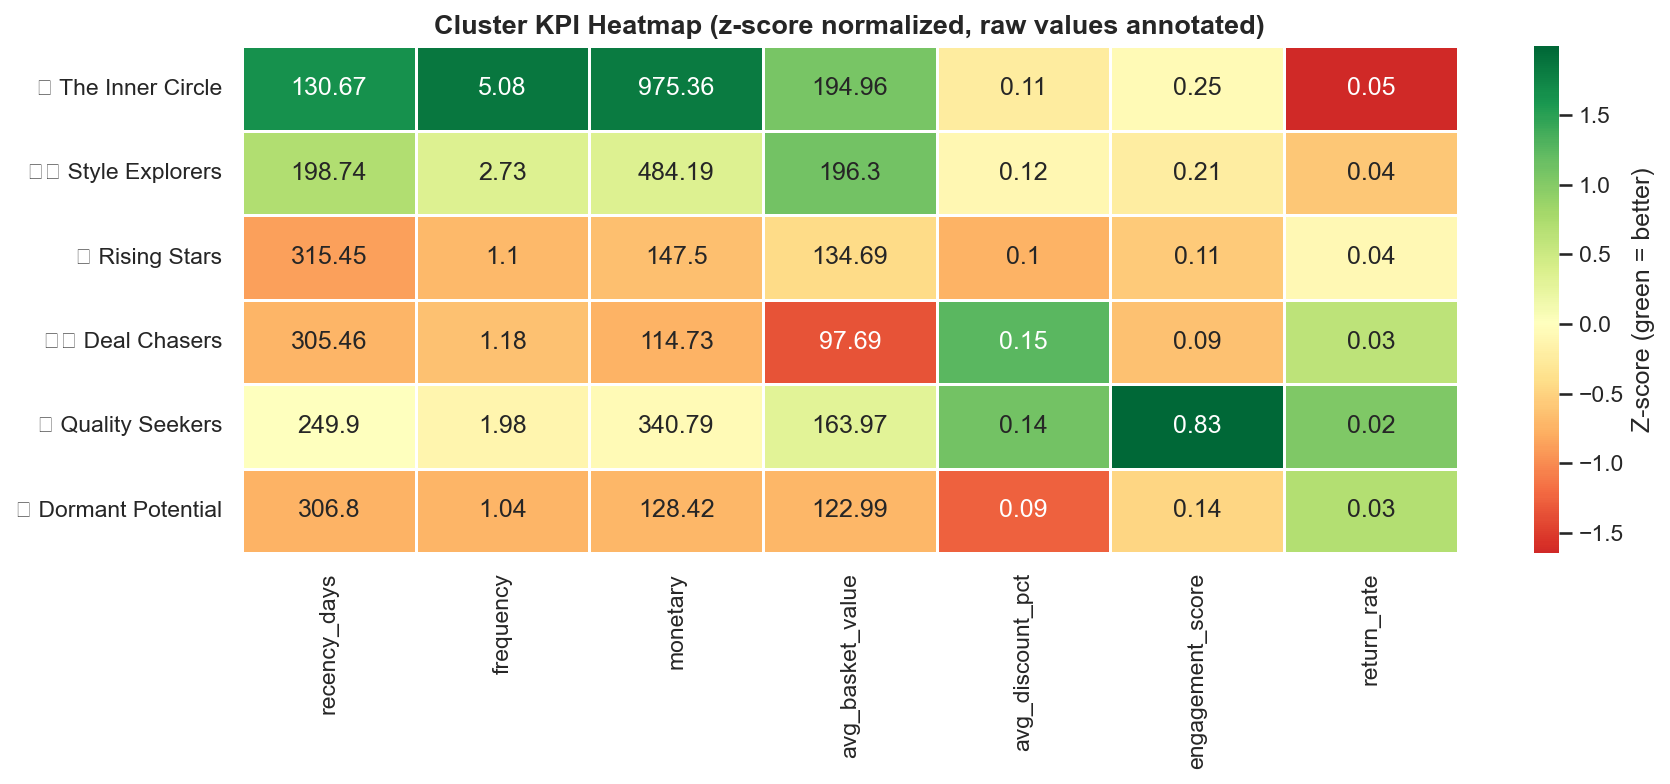
\includegraphics[width=\linewidth]{assets/cluster_heatmap.png}
  \caption{Normalised KPI heatmap (z-scores). Dominant dimension per segment:
    Active Loyalists (monetary + frequency), Core Customers (balanced moderate),
    One-Shot Shoppers (low frequency, low basket), Promo-Engaged (engagement),
    Lapsed Low-Value (high recency, low n), Churned (high recency, lowest activity).}
  \label{fig:heatmap}
\end{figure}

Figure~\ref{fig:heatmap} shows the normalised KPI heatmap: each segment has a dominant
feature dimension that distinguishes it from all others.

\textbf{Active Loyalists} ($n=6{,}495$, 30.3\%): the engaged core --- recent (avg
recency 131~days), high-frequency (5.0 visits over 24 months), high-monetary
(\eur957 cumulative, AOV \eur195) buyers with a low discount rate (11\%) and a
broad category footprint (avg 4.0 distinct categories). They generate 55.3\% of
\emph{projected annual run-rate revenue} (different metric than the 51.2\% Pareto
in \S\ref{ssec:eda}, which measures observed individual concentration), and
retention is a \textit{financial risk management} priority rather than a marketing
objective. A 5\,pp churn increase eliminates \eur228K of projected annual revenue ---
\$1.6\times$ the entire \eur140K strategic investment. The segment's dCLV of
\eur1,545 (2.8$\times$ Core Customers) quantifies the asymmetric value of protecting
each relationship. \textit{Proposed test}: VIP programme with automated churn-alert
at recency $>$90 days; validate on 12-month retention rate and CLV uplift vs.\ holdout.

\textbf{Core Customers} ($n=10{,}256$, 47.9\%): the volume-dominant segment ---
stable moderate-frequency buyers (2.7 visits over 24 months $\approx$ 1.36/yr,
AOV \eur192, monetary \eur484) without strong promotional dependency
(discount 12\%). Their moderate recency (199~days) and engagement (0.21) profile
indicates an active relationship that has not yet reached VIP maturity. Natural
feeder pool for Active Loyalists: even a 5\% upgrade rate would translate
\eur513 of stand-alone CLV per converted customer into the \eur1,545 tier ---
3.0$\times$ uplift on a $\sim$\eur30K gamification cost.
\textit{Proposed test}: gamified loyalty with visible tier-progress indicators
(``You are \eur{}X from VIP tier''); validate on tier-upgrade rate and 12-month AOV growth.

\textbf{One-Shot Shoppers} ($n=2{,}727$, 12.7\%): single-purchase customers
(frequency 1.18, n\_categories 1.14, AOV \eur98) who lapsed after one transaction
(avg recency 305~days). The defining signal is \emph{purchase shallowness}, not
category exploration: they bought from one category once and disengaged.
The strategy is therefore a \emph{2nd-purchase} conversion play rather than
a cross-category engine, with avg basket as the primary lever (\eur98 $\to$ \eur110
target via bundled cross-sell).
\textit{Proposed test}: ``Complete the Look'' email sequence at 30/60/90~days
post-first-purchase; validate on 2nd-purchase rate and basket size of
re-engaged customers.

\textbf{Promo-Engaged} ($n=768$, 3.6\%): the highest-engagement cluster
(\textbf{0.83 vs.\ portfolio average 0.23}, i.e.\ 3.7$\times$) --- an unusual
profile that combines high email open/click rates with above-average discount
sensitivity (14\%) and modest spend (monetary \eur341, AOV \eur163, freq 1.98).
This is the segment most responsive to communication; the strategic question is
\emph{whether to convert that engagement into discount dependency or into loyalty}.
The \eur20K allocation funds a controlled A/B (loyalty-points treatment vs.\
discount-email control) on randomised sub-groups; success is measured on net
margin per order, not gross revenue, since revenue uplift via discount is the
trivial counterfactual.
\textit{Proposed test}: discount email (control) vs.\ loyalty-bundle email
(treatment); validate on annual frequency (0.99 $\to$ 1.20/yr) and net margin.

\textbf{Lapsed Low-Value} ($n=675$, 3.2\%): dormant single-shot buyers (recency 315~d,
freq 1.10, monetary \eur148, n\_categories 1.00). Profile is near-identical
to \textit{Churned} on activity dimensions but with marginally higher spend ---
just enough to be worth a single low-cost reactivation attempt before suppression.
Reactivation cost is lower than cold acquisition (CRM data enables targeted
outreach), but positive ROI is not guaranteed; the proposed test partly serves
as a market research instrument to estimate reactivation elasticity for the
broader dormant tail.
\textit{Proposed test}: 3-touch win-back sequence at Day 30/60/90 post-last-purchase;
validate on 2nd-purchase rate at 90/180~days and 6-month LTV of reactivated cohort.

\textbf{Churned} ($n=503$, 2.3\%): the smallest cluster --- one-time, low-engagement
buyers (recency 306~d, freq 1.04, monetary \eur128, engagement 0.14). Distinct from
\textit{Lapsed Low-Value} in spend (\eur128 vs.\ \eur148) and basket structure but
otherwise behaviourally similar. Strategy is a \emph{minimum-viable} win-back: a
two-email sequence with a personalised re-engagement offer; if no response by
Day~60, the customer is moved to a suppression list to keep the active marketing
panel clean. \textit{Proposed test}: two-touch win-back vs.\ suppression-control;
validate on reactivation rate at 90~days and cost per reactivated customer.

\begin{figure}[H]
  \centering
  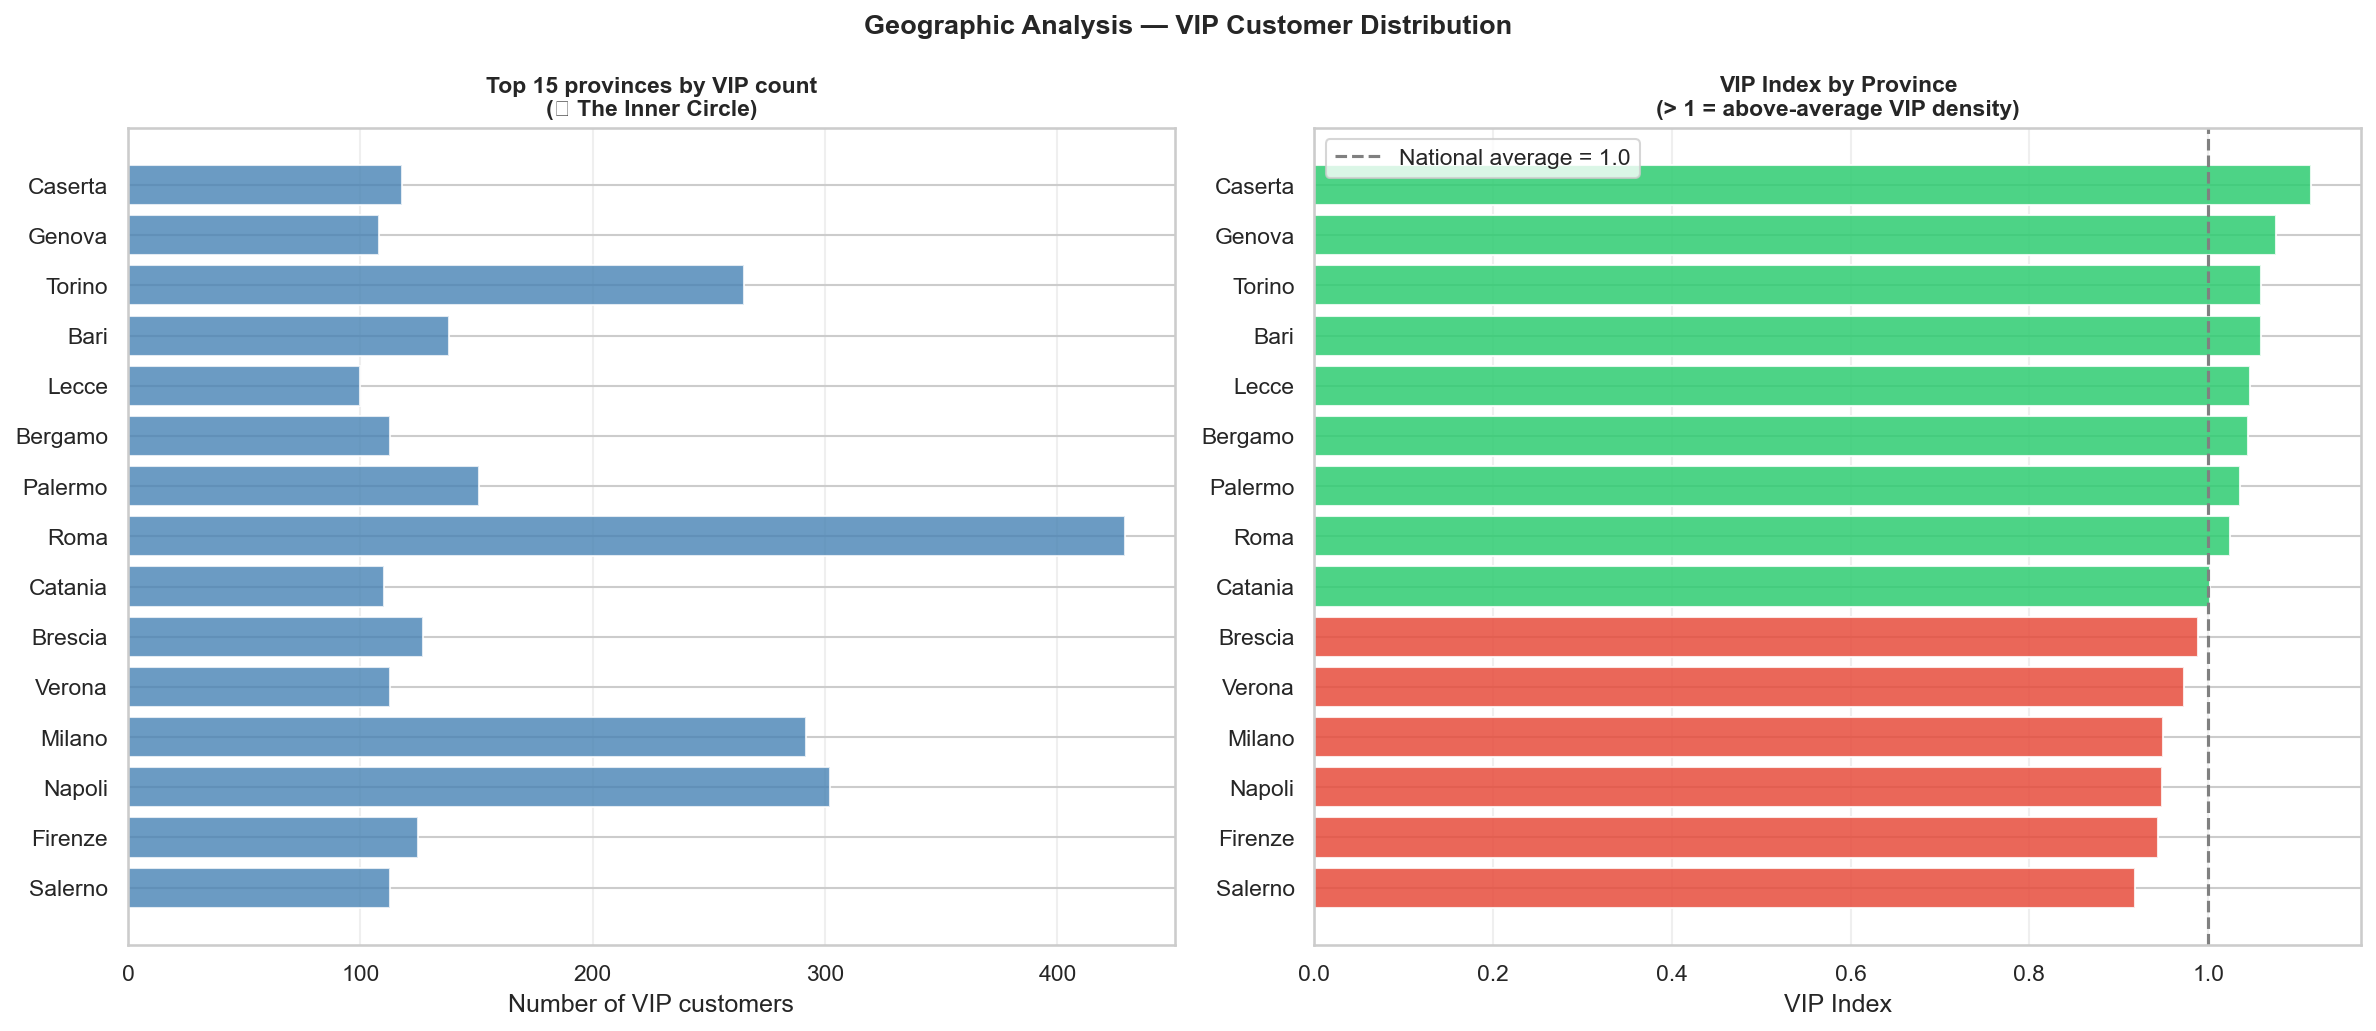
\includegraphics[width=0.88\linewidth]{assets/geo_vip.png}
  \caption{Geographic VIP index: province-level concentration of Active Loyalists
    relative to the provincial customer base. Darker provinces indicate above-average
    VIP density; three northern provinces account for $>$40\% of Active-Loyalist revenue,
    informing physical retail and event investment priorities.}
  \label{fig:geo}
\end{figure}

\subsection{Customer Lifetime Value}

Discounted CLV follows the constant-margin perpetuity model of Gupta \&
Lehmann \cite{gupta2003customers}:\footnote{Derivation: if a customer generates
$\mathrm{AOV}\!\times\!f_{\mathrm{annual}}$ per year and survives to the next
period with probability $r_{\mathrm{ret}}$, the expected discounted value of
future purchases is
$\mathrm{AOV}\!\times\!f \sum_{t=1}^{\infty}(r_{\mathrm{ret}}/(1+r))^t =
\mathrm{AOV}\!\times\!f\!\times\!r_{\mathrm{ret}}/(1\!+\!r\!-\!r_{\mathrm{ret}})$
(geometric series, $r_{\mathrm{ret}}/(1+r)<1$). This is a simplification: it
assumes a stationary purchase rate and a single annual retention probability,
and does not account for customer heterogeneity within segments (cf.\ the
BG/NBD model \cite{fader2005counting}).}
\begin{equation}
  \mathrm{dCLV} = \mathrm{AOV} \times f_{\mathrm{annual}}
    \times \frac{r_{\mathrm{ret}}}{1 + r - r_{\mathrm{ret}}},
    \qquad r = 0.10 \;\text{(WACC proxy).}
\label{eq:dclv}
\end{equation}
Per-segment $r_{\mathrm{ret}}$ is estimated as the observed repurchase rate:
the fraction of customers purchasing in both the first and second 12-month
sub-periods of the observation window. This is a proxy, not a steady-state
estimate; it is downward-biased for recently-acquired customers (see
limitations, Section~\ref{sec:conclusions}). The total portfolio CLV of
\textbf{\eur16,187,953} is a \textit{managerial stake measure}, not a
financial forecast. Figure~\ref{fig:clv} visualises the per-segment distribution.

\begin{figure}[H]
  \centering
  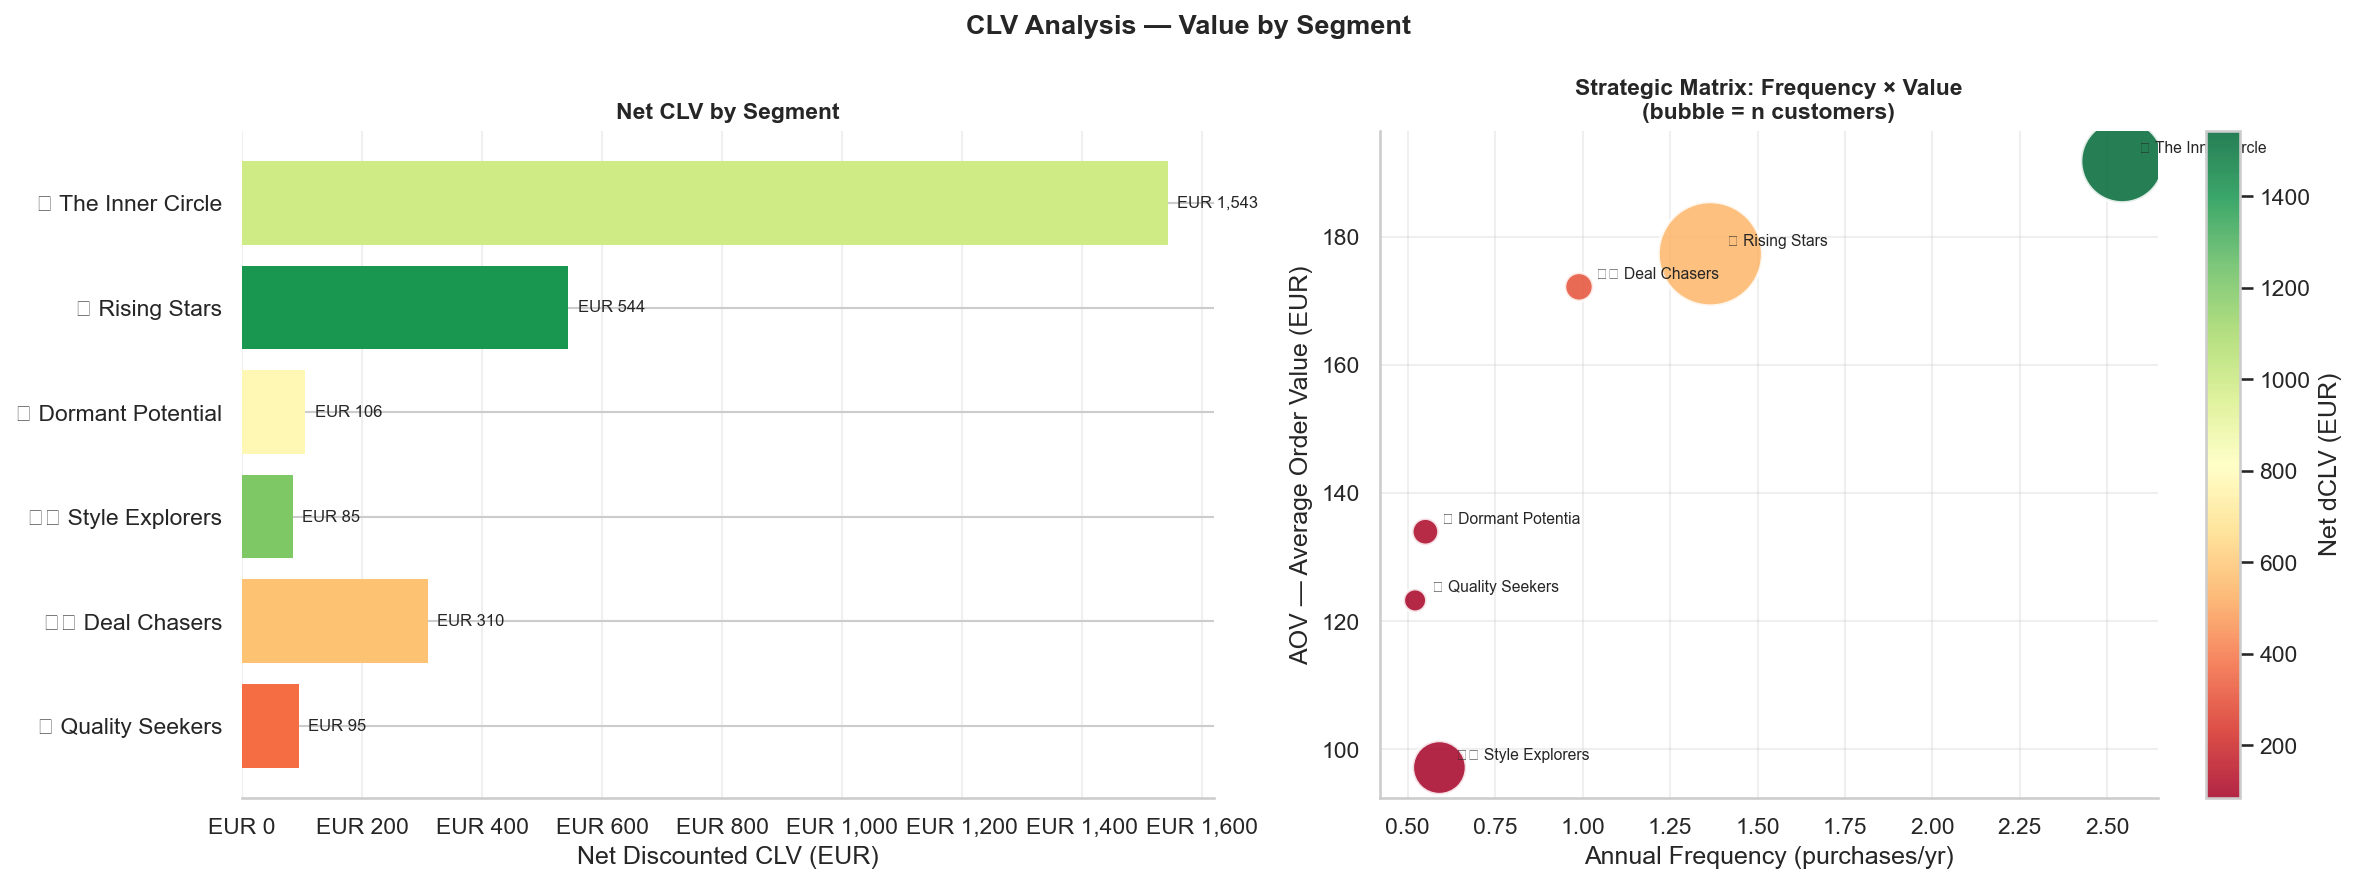
\includegraphics[width=\linewidth]{assets/clv_analysis.png}
  \caption{Discounted CLV by segment. Active Loyalists dCLV \eur1,545 vs.\ Core
    Customers \eur545 vs.\ tail segments $<$\eur310. Active Loyalists account for
    61.9\% of total portfolio dCLV from 30.3\% of customers.}
  \label{fig:clv}
\end{figure}

\subsection{Scenario ROI Framework}

Table~\ref{tab:roi} details the strategy matrix: each initiative is framed as a
testable hypothesis with an explicit behavioural assumption and a validation KPI.
Figure~\ref{fig:roi} visualises the decomposition of the \eur140K investment and
the corresponding scenario uplifts. Figure~\ref{fig:ceo} summarises the full CEO
P\&L heatmap.
The gross return multiple (ROI = Scenario Uplift / Annual Investment) is not an
accounting ROI: the uplifts derive from untested assumptions and carry no statistical
confidence bounds. They are intended to rank-order investment priorities, not to
forecast outcomes.

\begin{table}[H]
\centering\small
\caption{Scenario ROI matrix: initiatives framed as testable hypotheses.$^{b}$}
\label{tab:roi}
\begin{tabular}{@{}p{2.8cm}p{3.4cm}p{2.6cm}rrr@{}}
\toprule
\textbf{Segment} & \textbf{Proposed Initiative} & \textbf{Assumption}
  & \textbf{Budget} & \textbf{Uplift} & \textbf{ROI$^{b}$} \\
\midrule
Active Loyalists  & VIP programme + churn-alert & $-$5 pp churn
  & \eur45K & \eur228K & 5.1$\times$ \\
Core Customers    & Gamified loyalty tier       & 5\% upgrade rate
  & \eur30K & \eur95K  & 3.2$\times$ \\
One-Shot Shoppers & ``Complete the Look'' cross-sell & basket \eur98$\to$\eur110
  & \eur20K & \eur10K  & 0.5$\times$ \\
Promo-Engaged     & A/B loyalty vs.\ discount   & freq 0.99$\to$1.20/yr
  & \eur20K & \eur4K   & 0.2$\times$ \\
Lapsed Low-Value  & 3-touch win-back            & 15\% reactivation
  & \eur10K & \eur5K   & 0.5$\times$ \\
Churned           & 2-touch win-back / suppress & 6--8\% reactivation
  & \eur15K & \eur1K   & 0.1$\times$ \\
\midrule
\textbf{Total}  &                             &
  & \textbf{\eur140K} & \textbf{\eur342K} & \textbf{2.4$\times$} \\
\bottomrule
\end{tabular}
\vspace{2pt}\\
{\footnotesize $^{b}$ROI = gross return multiple = Scenario Uplift $\div$ Annual Investment.
\textit{Not} an accounting ROI; directional scenario estimates requiring A/B validation.\\[2pt]
\textit{Assumption benchmarks (base-case midpoints):}
($-$5\,pp churn): loyalty programmes in apparel report 2--8\,pp churn reduction
(McKinsey, ``The value of getting personalisation right'', 2021; \textbf{range: 2--8\,pp}).
($+$5\% conversion via gamification): digital loyalty tier experiments show 2--8\% uplift
(Hamari et al., ``Does Gamification Work?'', HICSS 2014; \textbf{range: 2--8\%}).
($+$15\% cross-sell): personalised recommendations drive 10--30\% incremental revenue in
apparel (McKinsey, ``The Next Normal'', 2020; \textbf{range: 5--20\%}).
($-$8\,pp return rate): digital size advisors reduce fashion returns by 5--15\,pp
(McKinsey State of Fashion 2023; \textbf{range: 4--12\,pp}).
All scenarios use base-case midpoints.}
\end{table}

\begin{figure}[H]
  \centering
  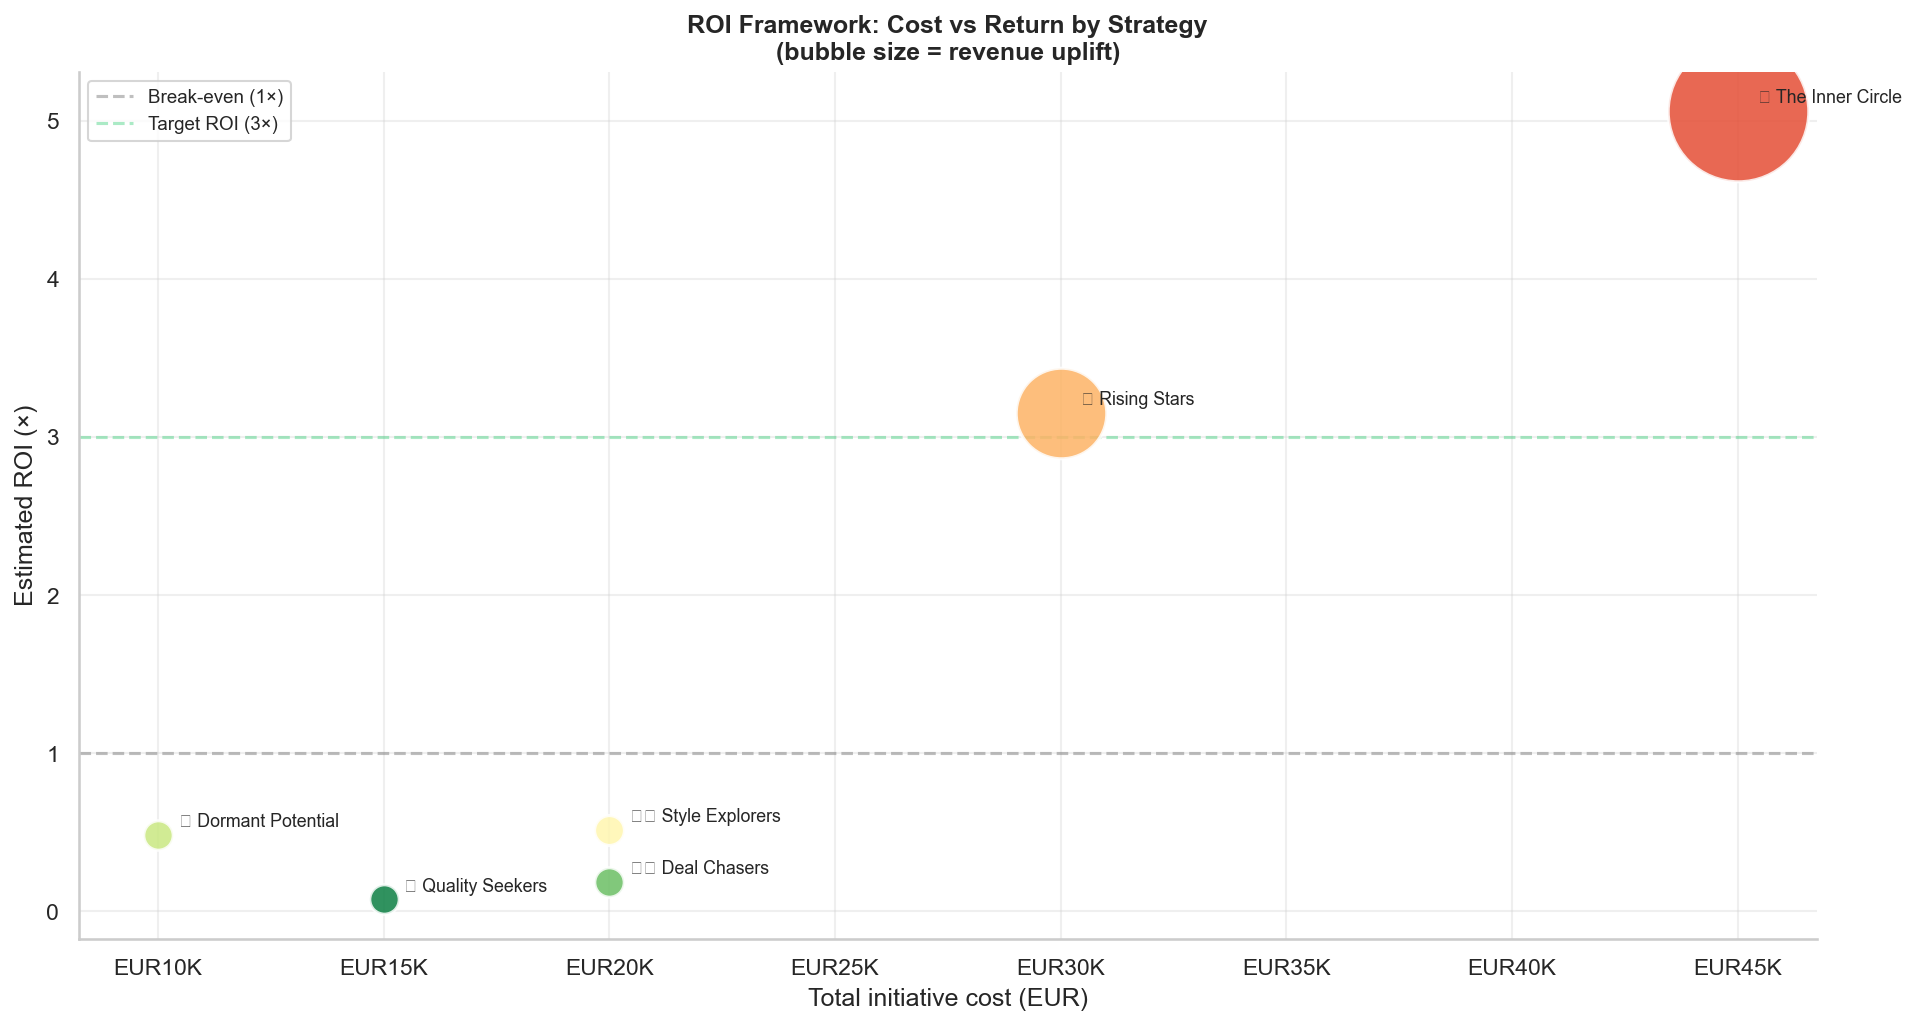
\includegraphics[width=\linewidth]{assets/roi_framework.png}
  \caption{Scenario ROI framework: investment allocation by segment (left), projected
    uplift (centre), gross return multiple (right). Active Loyalists (5.1$\times$) and
    Core Customers (3.2$\times$) account for \eur323K of the \eur342K total uplift.
    This is a \textit{concentrated-bet} strategy: two segments carry virtually all
    the expected return; four segments are learning investments with ROI $<$1$\times$.}
  \label{fig:roi}
\end{figure}

\begin{figure}[H]
  \centering
  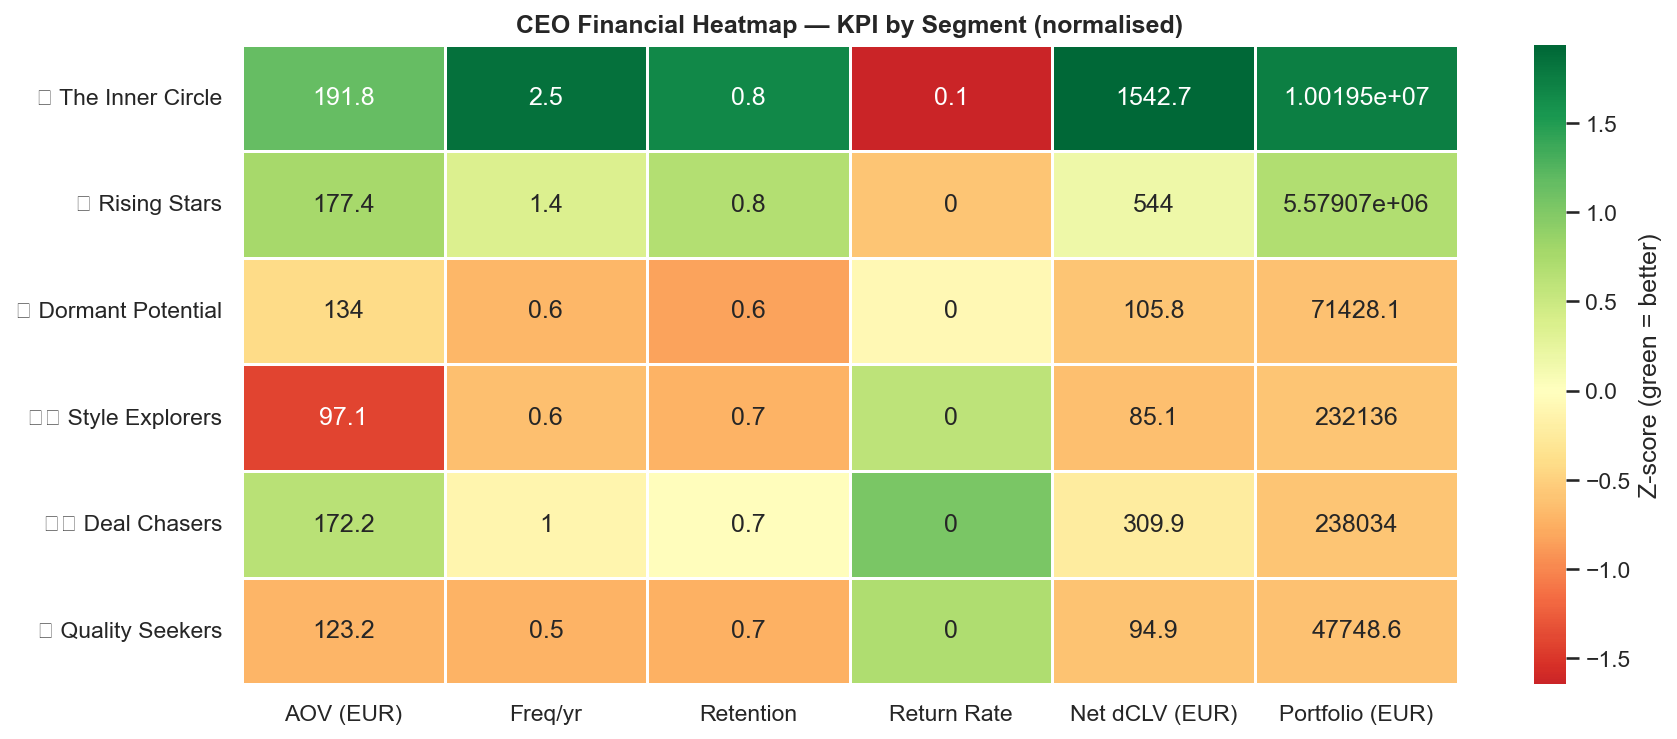
\includegraphics[width=\linewidth]{assets/ceo_pnl_heatmap.png}
  \caption{CEO P\&L heatmap: observed revenue, dCLV, portfolio CLV, and scenario ROI
    per segment. Active Loyalists and Core Customers account for 94.4\% of the
    \eur342K scenario uplift.}
  \label{fig:ceo}
\end{figure}

\begin{resultbox}
\small\textbf{Scenario financial summary} (directional; explicit assumptions in
Table~\ref{tab:roi}).\\[2pt]
Observed revenue (24-month): \textbf{\eur12,084,646}
$\;\cdot\;$ Portfolio CLV (NPV stake): \textbf{\eur16,187,953}
$\;\cdot\;$ Investment: \textbf{\eur140K/yr}
$\;\cdot\;$ Scenario uplift: \textbf{\eur342K/yr}
$\;\cdot\;$ Gross return multiple: \textbf{2.4$\times$}
$\;\cdot\;$ Implied payback: \textbf{$\sim$5 months}
\end{resultbox}

\begin{figure}[H]
  \centering
  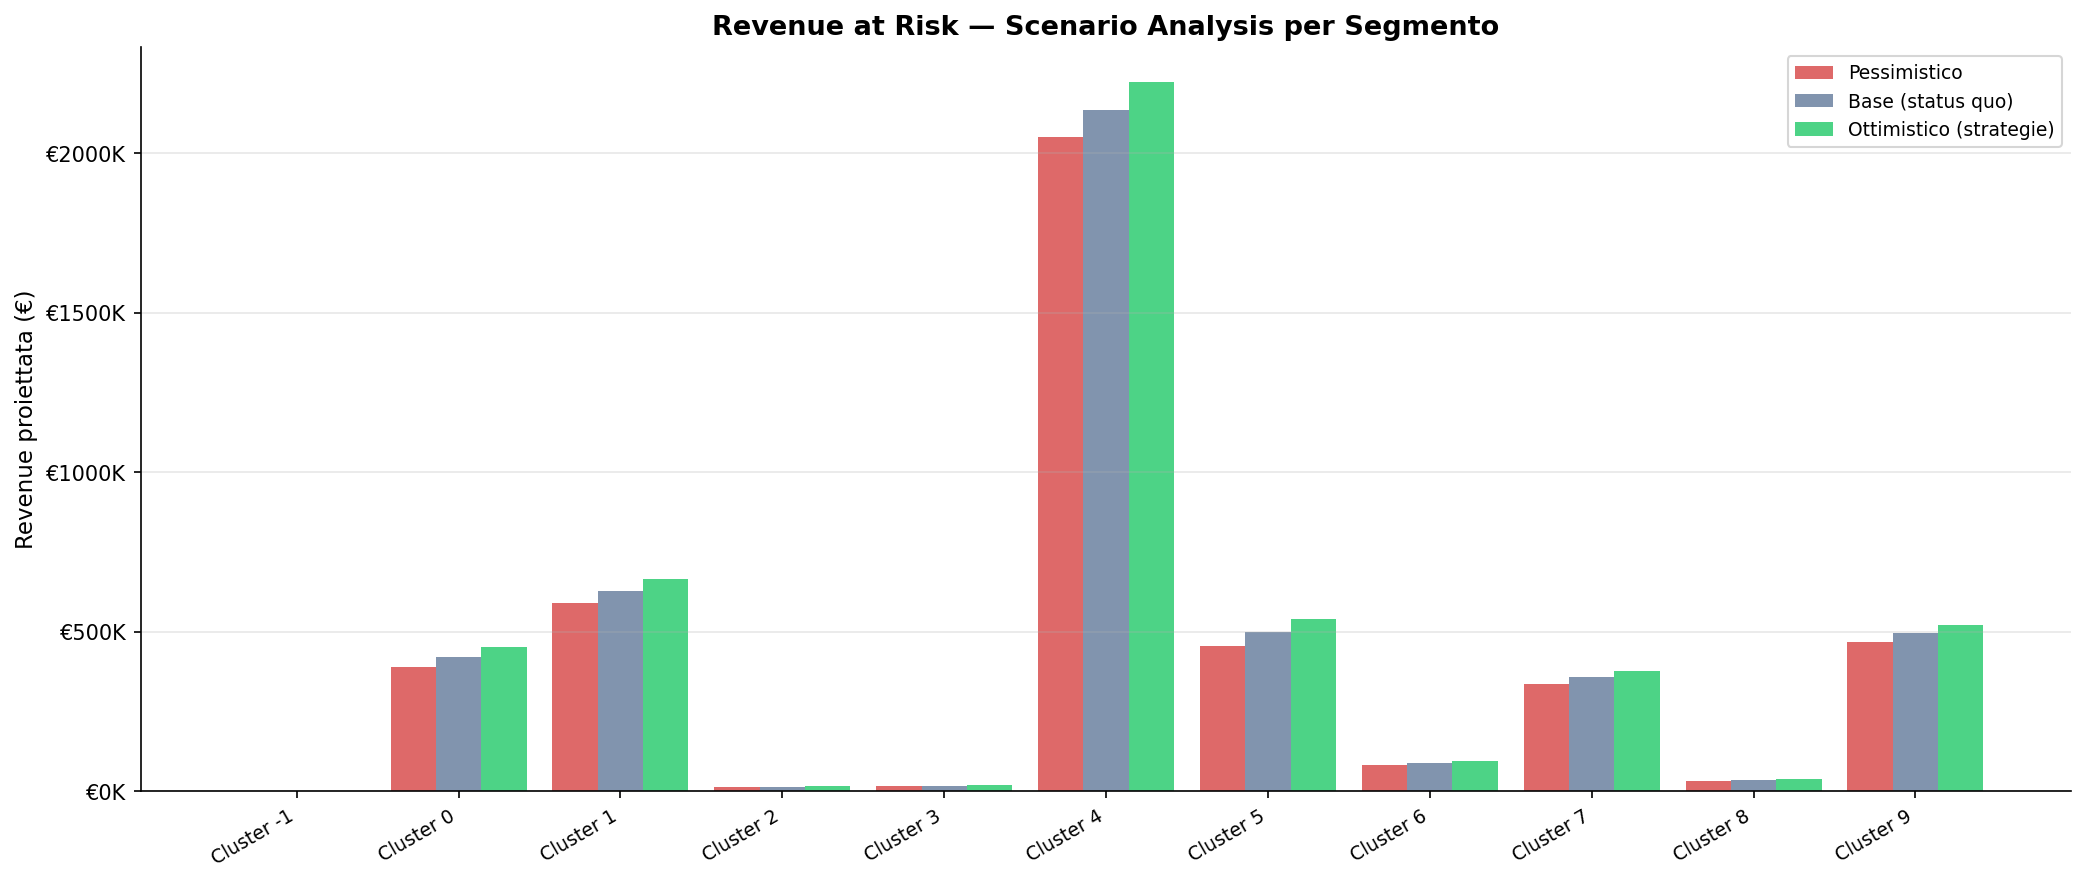
\includegraphics[width=\linewidth]{assets/revenue_at_risk.png}
  \caption{Revenue at Risk scenario: $\pm$20\% perturbation to observed churn rates per
    segment. Active Loyalists dominate the downside --- a 20\% churn increase generates
    the largest absolute revenue loss of any segment. Core Customers show the largest
    combined risk-and-opportunity profile given its size.}
  \label{fig:risk}
\end{figure}

\begin{keybox}
\small\textbf{Break-even sensitivity.}
The 2.4$\times$ portfolio multiple is driven by a concentrated bet: Active Loyalists
alone contribute \eur228K of \eur342K (66.7\%). The remaining five segments contribute
\eur114K against a combined \eur95K investment, but their individual ROIs are
$\leq$0.5$\times$. If the Active-Loyalist churn reduction falls below \textbf{0.6 pp}
(from the assumed 5 pp), the portfolio gross return multiple falls to $\leq 1\times$:
the VIP programme is therefore the single most consequential assumption to validate
first via a controlled A/B experiment.
\end{keybox}

\subsection{Sensitivity to Portfolio Scope}
\label{ssec:scope}

A legitimate challenge to the six-segment framework is whether concentrating budget
on the two high-ROI segments would deliver superior financial returns.
Table~\ref{tab:scope} compares the two scopes explicitly. \emph{Note on terminology}:
the ``concentrated portfolio'' below is \textbf{not} an alternative GMM solution
fitted at $K{=}2$ --- the underlying clustering remains the locked $K{=}6$ model.
The row simply restricts the strategy investment to the top two segments of that
solution, treating the other four as receiving zero strategic budget for the
purposes of the comparison.

\begin{table}[H]
\centering\small
\caption{Portfolio scope sensitivity: concentrated (top-2 segments of the $K{=}6$
solution) vs.\ full (all six segments of the same solution). The clustering model
is identical in both rows; only the budget allocation differs.}
\label{tab:scope}
\begin{tabular}{@{}lrrrr@{}}
\toprule
\textbf{Scope} & \textbf{Budget} & \textbf{Uplift} & \textbf{Gross ROI}
  & \textbf{Customers served} \\
\midrule
Concentrated portfolio (Active Loyalists + Core Customers only)
  & \eur75K  & \eur323K & 4.3$\times$ & 78.2\% \\
Full portfolio (all six segments)
  & \eur140K & \eur342K & 2.4$\times$ & 100\%  \\
\bottomrule
\end{tabular}
\end{table}

The concentrated allocation is more capital-efficient (4.3$\times$ vs.\ 2.4$\times$)
and covers 83.2\% of portfolio CLV. The full six-segment allocation adds three
returns absent from the concentrated ROI column: (i)~\textit{margin protection} ---
Promo-Engaged customers generate gross revenue but erode net margin through their
discount sensitivity, a benefit not captured as revenue uplift;
(ii)~\textit{early warning} --- Lapsed Low-Value growth is a leading indicator of
Active-Loyalist attrition (\eur10K/yr monitoring); (iii)~\textit{assumption
calibration} --- the four low-ROI experiments generate A/B evidence that validates
the \eur228K Active-Loyalist projection. \textbf{Practical recommendation:} if budget
is the binding constraint, the concentrated allocation delivers 94.4\% of projected
financial uplift at 54\% of the cost.

% ============================================================================
\section{Conclusions}
\label{sec:conclusions}
% ============================================================================

Three central conclusions emerge:

\begin{enumerate}
  \item \textbf{The customer base is structurally concentrated, but below the
    80/20 reference.} The top 20\% of individual customers generate 51.2\% of
    \emph{observed} revenue (Pareto, \S\ref{ssec:eda}); separately, the
    Active-Loyalist segment (30.3\% of customers) accounts for 55.3\% of
    \emph{projected annual run-rate revenue} and 61.9\% of total portfolio dCLV.
    The two metrics are complementary, not equivalent: the first is observed
    individual concentration, the second is forward-looking segment concentration.
    Both make Active-Loyalist retention a \textit{financial risk management}
    priority --- a 5\,pp churn increase in this single segment eliminates revenue
    of \eur228K, 1.6$\times$ the entire \eur140K strategic investment.
  \item \textbf{Behavioural segments prescribe qualitatively different levers.}
    Promo-Engaged and Active Loyalists both engage actively with the brand but require
    diametrically opposite interventions (discount-dependency mitigation vs.\
    retention insurance); One-Shot Shoppers and Lapsed Low-Value share dormant profiles
    but warrant different cost envelopes (cross-sell investment vs.\ low-touch
    reactivation). Segment-blind campaigns optimise for none of these. The six-segment
    framework provides the structural vocabulary for calibrated, non-uniform CRM
    treatment.
  \item \textbf{Analytical capability is a non-trivial intangible asset.}
    Economic value resides not in raw transactional data but in its transformation into
    a deployable segmentation framework \cite{corrado2009intangible,haskel2018capitalism}.
    The scenario projections remain directional pending A/B campaign outcomes;
    the segmentation model is immediately operational.
\end{enumerate}

\textbf{Operational Deployment Roadmap.}
The segmentation model is immediately operational for batch CRM scoring. A three-horizon
deployment plan is proposed:

\begin{enumerate}[topsep=2pt, itemsep=3pt]
  \item \textbf{Horizon 1 --- Month 1--3 (validate).}
    Deploy the segment labels to the CRM platform (via
    \texttt{customer\_segmentation\_results.csv}) and configure audience filters.
    Launch the Active-Loyalists VIP programme and Core-Customers tier-upgrade A/B
    test as the two highest-ROI initiatives. Collect holdout control groups for both.
    Establish a weekly monitoring dashboard tracking Silhouette Score on rolling
    24-month data.
  \item \textbf{Horizon 2 --- Month 4--6 (calibrate).}
    Analyse A/B results from Horizon 1. Update the \textbf{dCLV} model with
    empirically observed churn rates (replacing the estimated 12-month proxy).
    If observed Active-Loyalist churn reduction exceeds 0.6\,pp (break-even threshold),
    scale the VIP programme to the full segment. Extend experiments to One-Shot
    Shoppers (cross-sell engine) and Promo-Engaged (loyalty-points A/B).
  \item \textbf{Horizon 3 --- Quarterly retraining.}
    Retrain the full pipeline on a rolling 24-month window every quarter, or
    immediately if: (a) segment size distribution shifts $>$10\% vs.\ prior quarter,
    (b) Silhouette Score drops below 0.34, or (c) the retailer adds a new product
    category that materially changes the category-affinity feature space.
    Inference for new customers is possible without retraining (see Appendix~A).
\end{enumerate}

\textbf{Limitations.}
(i)~\textit{Financial projections are unvalidated}: CLV, Revenue at Risk, and ROI
estimates are decision-support tools, not audited forecasts; controlled A/B experiments
are required before operational adoption.
(ii)~\textit{Temporal selection bias}: customers acquired late in the window have fewer
months of history, potentially underestimating their true purchase rate.
(iii)~\textit{Single-retailer scope}: segments are data-specific; the methodology
transfers to new datasets, but segments must be re-derived from scratch.
(iv)~\textit{UMAP stochasticity}: despite \texttt{random\_state=42}, minor numerical
non-determinism may shift segment boundaries slightly across hardware environments.
(v)~\textit{CLV model simplifications}: the constant-margin perpetuity formula assumes
a stationary annual purchase rate and ignores within-segment heterogeneity; the
BG/NBD model \cite{fader2005counting} would provide more granular individual-level
CLV estimates but requires individual-level calibration data and substantially
greater computational infrastructure.
(vi)~\textit{Missing channels}: the current feature set captures email engagement
but not social media or in-store advisor interactions. As omnichannel data becomes
available, the 24-feature matrix should be extended and the pipeline rerun to
assess whether additional segments emerge (particularly a \textit{Social Shopper}
profile not separable from current data).

% ============================================================================
{\small
\begin{thebibliography}{99}
\setlength{\itemsep}{1pt}
\bibitem{bellman1961adaptive}
  Bellman, R. (1961). \textit{Adaptive Control Processes: A Guided Tour}.
  Princeton University Press.
\bibitem{bult1995optimal}
  Bult, J.R.\ \& Wansbeek, T. (1995). Optimal selection for direct mail.
  \textit{Marketing Science}, 14(4), 378--394.
\bibitem{corrado2009intangible}
  Corrado, C., Hulten, C.\ \& Sichel, D. (2009). Intangible capital and U.S.\ economic
  growth. \textit{Review of Income and Wealth}, 55(3), 661--685.
\bibitem{dempster1977}
  Dempster, A.P., Laird, N.M.\ \& Rubin, D.B. (1977). Maximum likelihood from
  incomplete data via the EM algorithm. \textit{J.\ Royal Statistical Society B},
  39(1), 1--22.
\bibitem{fader2005counting}
  Fader, P.S., Hardie, B.G.S.\ \& Lee, K.L. (2005). Counting your customers the easy way.
  \textit{Marketing Science}, 24(2), 275--284.
\bibitem{gupta2003customers}
  Gupta, S.\ \& Lehmann, D.R. (2003). Customers as assets.
  \textit{Journal of Interactive Marketing}, 17(1), 9--24.
\bibitem{gupta2006modeling}
  Gupta, S.\ \& Zeithaml, V. (2006). Customer metrics and their impact on financial
  performance. \textit{Marketing Science}, 25(6), 718--739.
\bibitem{haskel2018capitalism}
  Haskel, J.\ \& Westlake, S. (2018). \textit{Capitalism Without Capital}.
  Princeton University Press.
\bibitem{kaufman1990finding}
  Kaufman, L.\ \& Rousseeuw, P.J. (1990).
  \textit{Finding Groups in Data: An Introduction to Cluster Analysis}. Wiley.
\bibitem{kriegel2011density}
  Kriegel, H.P., Kr\"{o}ger, P., Sander, J.\ \& Zimmer, A. (2011).
  Density-based clustering.
  \textit{WIREs Data Mining and Knowledge Discovery}, 1(3), 231--240.
\bibitem{mcinnes2018umap}
  McInnes, L., Healy, J.\ \& Melville, J. (2018).
  UMAP: Uniform Manifold Approximation and Projection. \textit{arXiv:1802.03426}.
\bibitem{pedregosa2011scikit}
  Pedregosa, F.\ et al.\ (2011). Scikit-learn: Machine Learning in Python.
  \textit{JMLR}, 12, 2825--2830.
\bibitem{wedel2000market}
  Wedel, M.\ \& Kamakura, W. (2000).
  \textit{Market Segmentation: Conceptual and Methodological Foundations} (2nd ed.).
  Kluwer Academic.
\end{thebibliography}
}

% ============================================================================
\appendix
\titleformat{\section}{\large\bfseries\color{navy}}{Appendix~\Alph{section}}{0.6em}{}
  [{\color{accent}\titlerule[0.4pt]}]
\titlespacing{\section}{0pt}{6pt}{2pt}

\section{Code Description}
\label{app:code}
% ============================================================================

\textbf{Pipeline overview.} The six CRISP-DM phases map to seven implementation
steps in \texttt{master\_segmentation.ipynb} (39 cells): steps 1--2 cover Data
Understanding/Preparation; steps 3--5 cover Modelling; step 6 covers Evaluation;
step 7 is a \textit{Financial Extension} (not a canonical CRISP-DM phase) that
produces the CLV and ROI outputs. Two helper modules support the pipeline:
\texttt{src/data\_processing.py} (feature engineering) and
\texttt{src/clustering\_model.py} (scaling, UMAP, GMM, evaluation). All I/O
is routed through \texttt{src/io/}.

\vspace{4pt}
\begin{center}
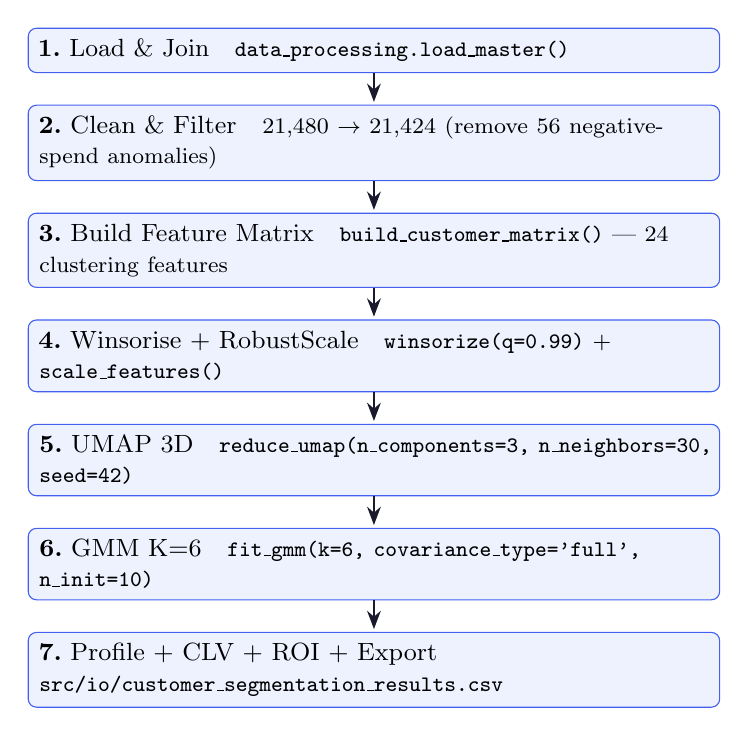
\begin{tikzpicture}[
  node distance=0.40cm,
  box/.style={rectangle, rounded corners=3pt, draw=accent, fill=boxbg,
    text width=8.5cm, align=left, font=\small, inner sep=4pt},
  arr/.style={-Stealth, thick, color=navy, shorten >=1pt}
]
\node[box] (load)  {\textbf{1.}\ Load \& Join\quad
  {\footnotesize\texttt{data\_processing.load\_master()}}};
\node[box, below=of load]  (clean) {\textbf{2.}\ Clean \& Filter\quad
  {\footnotesize 21,480 $\to$ 21,424 (remove 56 negative-spend anomalies)}};
\node[box, below=of clean] (feat)  {\textbf{3.}\ Build Feature Matrix\quad
  {\footnotesize\texttt{build\_customer\_matrix()} — 24 clustering features}};
\node[box, below=of feat]  (scale) {\textbf{4.}\ Winsorise + RobustScale\quad
  {\footnotesize\texttt{winsorize(q=0.99)} + \texttt{scale\_features()}}};
\node[box, below=of scale] (umap)  {\textbf{5.}\ UMAP 3D\quad
  {\footnotesize\texttt{reduce\_umap(n\_components=3, n\_neighbors=30, seed=42)}}};
\node[box, below=of umap]  (gmm)   {\textbf{6.}\ GMM K=6\quad
  {\footnotesize\texttt{fit\_gmm(k=6, covariance\_type='full', n\_init=10)}}};
\node[box, below=of gmm]   (out)   {\textbf{7.}\ Profile + CLV + ROI + Export\quad
  {\footnotesize\texttt{src/io/customer\_segmentation\_results.csv}}};
\draw[arr] (load.south) -- (clean.north);
\draw[arr] (clean.south) -- (feat.north);
\draw[arr] (feat.south) -- (scale.north);
\draw[arr] (scale.south) -- (umap.north);
\draw[arr] (umap.south) -- (gmm.north);
\draw[arr] (gmm.south) -- (out.north);
\end{tikzpicture}
\end{center}

\vspace{3pt}
\textbf{Inference pseudocode for new customers:}
\begin{verbatim}
x_new = build_feature_vector(new_customer_transactions)   # 24 features
x_sc  = scaler.transform(x_new)           # RobustScaler (src/io/models/scaler.pkl)
z     = reducer_3d.transform(x_sc)         # UMAP 3D  (src/io/models/reducer_umap3d.pkl)
k_hat = gmm.predict(z)                     # Segment assignment
p_k   = gmm.predict_proba(z)               # Confidence score  (src/io/models/gmm_k6.pkl)
# Deploy only to customers with p_k > 0.80 in first CRM wave
\end{verbatim}

\textbf{Re-training trigger:} quarterly rolling 24-month window, or immediately if
segment size distribution drifts $>$10\% or Silhouette drops below 0.34.

% ============================================================================
\section{Author Contribution (CRediT) and GenAI Statement}
\label{app:credit}
% ============================================================================

\textbf{CRediT Author Contributions.}

\vspace{4pt}
\noindent
\begin{tabular}{@{}p{4.2cm}p{9.0cm}@{}}
\toprule
\textbf{Contributor} & \textbf{CRediT Roles} \\
\midrule
$\langle\langle$INSERIRE NOME$\rangle\rangle$ &
  Conceptualisation; Methodology; Software; Formal analysis;
  Writing --- original draft \\[3pt]
$\langle\langle$INSERIRE NOME$\rangle\rangle$ &
  Methodology; Visualisation; Writing --- review \& editing \\[3pt]
$\langle\langle$INSERIRE NOME$\rangle\rangle$ &
  Data Curation; Validation; Writing --- review \& editing \\[3pt]
$\langle\langle$INSERIRE NOME$\rangle\rangle$ &
  Project administration; Investigation; Writing --- review \& editing \\
\bottomrule
\end{tabular}

\vspace{8pt}
\textbf{Generative AI Statement.}
Generative AI tools (Claude Sonnet 4.x, ChatGPT-4o) were used in this project
exclusively for: (i)~code debugging and refactoring of Python helper modules in
\texttt{src/}; (ii)~proofreading and grammar correction of written text. All
analytical decisions, quantitative results, and conclusions are the sole
responsibility of the authors. No AI-generated text appears verbatim in this
report. All figures, tables, and numerical outputs were produced by executing
\texttt{master\_segmentation.ipynb} directly on the original dataset provided by
Jakala S.p.A.

\end{document}
